\documentclass[]{article}
\usepackage{lmodern}
\usepackage{amssymb,amsmath}
\usepackage{ifxetex,ifluatex}
\usepackage{fixltx2e} % provides \textsubscript
\ifnum 0\ifxetex 1\fi\ifluatex 1\fi=0 % if pdftex
  \usepackage[T1]{fontenc}
  \usepackage[utf8]{inputenc}
\else % if luatex or xelatex
  \ifxetex
    \usepackage{mathspec}
  \else
    \usepackage{fontspec}
  \fi
  \defaultfontfeatures{Ligatures=TeX,Scale=MatchLowercase}
\fi
% use upquote if available, for straight quotes in verbatim environments
\IfFileExists{upquote.sty}{\usepackage{upquote}}{}
% use microtype if available
\IfFileExists{microtype.sty}{%
\usepackage{microtype}
\UseMicrotypeSet[protrusion]{basicmath} % disable protrusion for tt fonts
}{}
\usepackage[margin=1in]{geometry}
\usepackage{hyperref}
\hypersetup{unicode=true,
            pdftitle={Parcial 1: Biodisponibilidad y Bioequivalencia 2018-01},
            pdfauthor={Parra G., Daniel S.},
            pdfborder={0 0 0},
            breaklinks=true}
\urlstyle{same}  % don't use monospace font for urls
\usepackage{longtable,booktabs}
\usepackage{graphicx,grffile}
\makeatletter
\def\maxwidth{\ifdim\Gin@nat@width>\linewidth\linewidth\else\Gin@nat@width\fi}
\def\maxheight{\ifdim\Gin@nat@height>\textheight\textheight\else\Gin@nat@height\fi}
\makeatother
% Scale images if necessary, so that they will not overflow the page
% margins by default, and it is still possible to overwrite the defaults
% using explicit options in \includegraphics[width, height, ...]{}
\setkeys{Gin}{width=\maxwidth,height=\maxheight,keepaspectratio}
\IfFileExists{parskip.sty}{%
\usepackage{parskip}
}{% else
\setlength{\parindent}{0pt}
\setlength{\parskip}{6pt plus 2pt minus 1pt}
}
\setlength{\emergencystretch}{3em}  % prevent overfull lines
\providecommand{\tightlist}{%
  \setlength{\itemsep}{0pt}\setlength{\parskip}{0pt}}
\setcounter{secnumdepth}{0}
% Redefines (sub)paragraphs to behave more like sections
\ifx\paragraph\undefined\else
\let\oldparagraph\paragraph
\renewcommand{\paragraph}[1]{\oldparagraph{#1}\mbox{}}
\fi
\ifx\subparagraph\undefined\else
\let\oldsubparagraph\subparagraph
\renewcommand{\subparagraph}[1]{\oldsubparagraph{#1}\mbox{}}
\fi

%%% Use protect on footnotes to avoid problems with footnotes in titles
\let\rmarkdownfootnote\footnote%
\def\footnote{\protect\rmarkdownfootnote}

%%% Change title format to be more compact
\usepackage{titling}

% Create subtitle command for use in maketitle
\newcommand{\subtitle}[1]{
  \posttitle{
    \begin{center}\large#1\end{center}
    }
}

\setlength{\droptitle}{-2em}

  \title{Parcial 1: Biodisponibilidad y Bioequivalencia 2018-01}
    \pretitle{\vspace{\droptitle}\centering\huge}
  \posttitle{\par}
    \author{Parra G., Daniel S.}
    \preauthor{\centering\large\emph}
  \postauthor{\par}
      \predate{\centering\large\emph}
  \postdate{\par}
    \date{19 de septiembre de 2018}

\usepackage[spanish,es-nodecimaldot]{babel}
\usepackage{float}
\usepackage{fancyhdr}
\pagestyle{fancy}
\fancyhead[CO,CE]{}
\fancyfoot[CO,CE]{Departamento de Farmacia, Biodisponibilidad y Bioequivalencia}
\fancyfoot[LE,RO]{\thepage}

\begin{document}
\maketitle

\section{1. Enunciado}\label{enunciado}

Se ha efectuado un estudio para demostrar la bioequivalencia entre dos
productos que llevan como principio activo Antibiótico SP-4X el que se
prescribe a razón de 140 mg por vía IV y 700 mg por vía oral en
presentación de tabletas. Para el estudio se utilizó un diseño
experimental cruzado con 12 voluntarios, los que se dividieron en 2
grupos de 6 voluntarios, quienes recibieron en periodos diferentes los
dos productos en estudio (referencia y competidor). El estudio estuvo
completamente controlado los voluntarios fueron todos hombres con edades
comprendidas entre los 20 y 35 años y con un peso promedio de 70
kilogramos, la alimentación fue estandarizada y el producto se
administró en ayunas con 250 mL de agua, después de 10 horas de ayuno.
Del análisis de las muestras de sangre, por un método bioanalítico
validado, se obtuvieron los datos que se indican a continuación y se
solicita calcular:

\begin{enumerate}
\def\labelenumi{\arabic{enumi}.}
\item
  La constante de velocidad de eliminación (\(k_{e}\)) del antibiótico
  en la muestra poblacional utilizada, datos individuales y el promedio
  poblacional con su variabilidad (emplear la constante determinada por
  la vía IV en los cálculos subsiguientes de AUC\(|_{0}^{\infty}\)).
\item
  Determinar la constante de velocidad de absorción para el fármaco en
  los dos productos. Datos individuales y el promedio poblacional con su
  variabilidad (emplear la constante correspondiente a cada producto
  para los cálculos del \(C_{max}\) y del \(t_{max}\)).
\item
  Calcule y tabule los parámetros biofarmacéuticos para cada producto en
  cada individuo y establezca el valor medio (\(\bar{\theta}\)) y su
  variabilidad, ilustre los resultados con las gráficas correspondientes
  para cada individuo con los dos productos (una sóla gráfica para los
  12 individuos de un mismo producto). Establezca la gráfica promedio
  poblacional para cada producto (En esta se compara en una misma los
  dos productos).
\item
  ¿Cuál es la biodisponibilidad \(F\) de cada producto?
\item
  Se podrían considerar bioequivalentes los dos productos, ¿por qué?
  Justifique plenamente su respuesta.
\end{enumerate}

\section{2. Etapa de Modelamiento}\label{etapa-de-modelamiento}

\subsection{2.1. Modelamiento Individual Datos Administración
IV}\label{modelamiento-individual-datos-administracion-iv}

Se han modelado mediante regresión no-lineal los datos de
concentración-tiempo para el producto de referencia tras admistración
intravenosa (IV). El modelo farmacocinético para estos datos corresponde
a modelo de 1 compartimento que se describe de manera general por
ecuaciones diferenciales:

\[
\left\{\begin{matrix}
\begin{aligned}
&\frac{dx_{1}(t)}{dt} = -k_{e}x_{1}(t)+k_{a}x_{2}(t)+r(t) \\ 
\\
&\frac{dx_{2}(t)}{dt} = -k_{a}x_{2}(t) 
\end{aligned}
\end{matrix}\right.
\] En una forma matricial es equivalente a la siguiente expresión:\\
\[\frac{\mathrm{d} \vec{x}}{\mathrm{d} t} = \frac{\mathrm{d} }{\mathrm{d} t} \begin{bmatrix} x_{1}(t)\\ x_{2}(t) \end{bmatrix} = \begin{bmatrix} -k_{e} & k_{a} \\ 0 & -k_{a} \end{bmatrix} \cdot \begin{bmatrix}x_{1}(t)\\x_{2}(t)\end{bmatrix} + \begin{bmatrix}r(t)\\0\end{bmatrix}\]
En este caso \(x_{1}\) y \(x_{2}\) son las cantidades en los
compartimentos 1 (central), y 2 (absorción) en unidades de masa. De esta
se puede obtener la concentración plasmática \(C_{P}\) al dividir la
cantidad en el compartimento central \(x_{1}\) sobre el volumen de
distribución \(V_{D}\). Las constantes de velocidad \(k_{a}\) y
\(k_{e}\) son de absorción y eliminación respectivamente, el término
\(r(t)\) se añade para denotar un aporte de fármaco al sistema de primer
órden (p.~ej. en el caso de infusión continua).

En el caso de administración IV en forma de bolo simple, se puede
resolver la ecuación de manera analítica relacionando \(C_{p}\) y
tiempo. Al tener en cuenta también el error residual, se tiene el
siguiente modelo no lineal:

\[\vec{C_{p}} = \frac{D_{0}}{V_{D}}\cdot  e^{-k_{e}\cdot \vec{t}} + \vec{\varepsilon} \qquad \varepsilon_{i}\sim \mathcal{N}(0,\,\sigma^{2})\]

En este caso se tiene que \(\vec{C_{p}}\) es el vector de
concentraciones plasmáticas observadas, mientras \(\vec{t}\) es un
vector que corresponde a los tiempos en los cuales se han medido las
concentraciones. Se tiene que \(D_{0}\) es la dosis administrada en
bolo, y \(\vec{\varepsilon}\) es un vector con residuales que se definen
como la diferencia entre las concentraciones plasmáticas observadas
menos las predichas por el modelo. Los residuales se distribuyen de
manera nomal alrededor de cero con varianza \(\sigma^{2}\). El modelo
está parametrizado con \(k_{e}\) y \(V_{D}\), y se pueden obtener
parámetros secundarios como clearance total
\(CL_{T} = k_{e} \cdot V_{D}\), concentración inicial
\(C_{0} = \frac{D_{0}}{V_{D}}\), y tiempo de vida media
\(t_{1/2} = \ln{2}/k_{e}\).

El área bajo la curva truncada y total se obtienen al sumar las áreas
por el método de trapezoides, que se define para un intervalo de tiempo
entre el primer punto y el último punto de muestreo (\(C_{p}^{*}\)):\\
\[\textrm{AUC}_{\textrm{TRUNC}} = \left(\frac{ \left[ C_{0}+C_{p}(t_{1})\right ]}{2} \cdot t_{1}\right ) + \sum_{i=1}^{n-1}{ \frac{\left [C_{p}(t_{i})+C_{p}(t_{i+1})\right ]}{2} \cdot (t_{i+1}-t_{i})}\]

El área bajo la curva total se define por medio de la siguiente
expresión:\\
\[\textrm{AUC} = \left(\frac{\left[ C_{0}+C_{p}(t_{1}) \right ]}{2} \cdot t_{1}\right ) + \sum_{i=1}^{n-1}{ \frac{\left[ C_{p}(t_{i})+C_{p}(t_{i+1})\right]}{2} \cdot (t_{i+1}-t_{i})} + \frac{C_{p}(t_{n})}{k_{e}}\]\\
El modelamiento se ha realizado por medio del algoritmo de Gauss-Newton,
la función objetivo tiene la forma de suma de errores al cuadrado
\(S(\theta) = \sum_{i=1}^{n}{\varepsilon_{i}^2}\), como no tiene una
solución analítica se realiza un procedimiento de optimización. Las
variables de optimización son 50 iteraciones máximo, criterio de
tolerancia \textless{}1E-05, sin límites para los parámetros, y con
valor de ascenso de 1/1024. En el cuadro 1, se puede observar un reporte
de los resultados de modelamiento para los datos de administración
intravenosa.

\begin{longtable}[]{@{}ccccccccc@{}}
\caption{Resultados de Regresión Modelos 1 Compartimento (Producto
IV)}\tabularnewline
\toprule
ID & Dosis & \(V_{D}\) & \(k_{e}\) & \(CL_{T}\) & \(C_{0}\) &
\(t_{1/2}\) & AUC\(_{0}^{C_{P}^{*}}\) &
AUC\(_{0}^{\infty}\)\tabularnewline
\midrule
\endfirsthead
\toprule
ID & Dosis & \(V_{D}\) & \(k_{e}\) & \(CL_{T}\) & \(C_{0}\) &
\(t_{1/2}\) & AUC\(_{0}^{C_{P}^{*}}\) &
AUC\(_{0}^{\infty}\)\tabularnewline
\midrule
\endhead
Sujeto 01 & 140 & 21.005 & 0.230 & 4.828 & 6.665 & 3.015 & 27.374 &
29.201\tabularnewline
Sujeto 02 & 140 & 20.385 & 0.230 & 4.688 & 6.868 & 3.013 & 28.192 &
30.062\tabularnewline
Sujeto 03 & 140 & 21.663 & 0.230 & 4.976 & 6.463 & 3.017 & 26.556 &
28.341\tabularnewline
Sujeto 04 & 140 & 19.995 & 0.230 & 4.602 & 7.002 & 3.011 & 28.720 &
30.632\tabularnewline
Sujeto 05 & 140 & 22.122 & 0.230 & 5.077 & 6.329 & 3.019 & 26.027 &
27.770\tabularnewline
Sujeto 06 & 140 & 21.879 & 0.230 & 5.032 & 6.399 & 3.013 & 26.265 &
28.004\tabularnewline
Sujeto 07 & 140 & 20.198 & 0.230 & 4.640 & 6.931 & 3.017 & 28.483 &
30.398\tabularnewline
Sujeto 08 & 140 & 19.449 & 0.230 & 4.474 & 7.198 & 3.013 & 29.532 &
31.488\tabularnewline
Sujeto 09 & 140 & 22.845 & 0.230 & 5.246 & 6.128 & 3.018 & 25.190 &
26.888\tabularnewline
Sujeto 10 & 140 & 20.388 & 0.234 & 4.778 & 6.867 & 2.957 & 27.702 &
29.537\tabularnewline
Sujeto 11 & 140 & 22.129 & 0.231 & 5.104 & 6.327 & 3.005 & 25.949 &
27.727\tabularnewline
Sujeto 12 & 140 & 21.917 & 0.232 & 5.083 & 6.388 & 2.988 & 26.027 &
27.665\tabularnewline
\bottomrule
\end{longtable}

En la figura 1 se pueden observar los perfiles farmacocinéticos
(concentración-tiempo) de cada individuo con el ajuste del modelo. En el
cuadro 2 se observan tres parámetros de bondad de ajuste del modelo
coeficiente de determinación (\(R^{2}\)), grados de libertad
(\(g_{L}\)), y error residual estándar (\(\textrm{RSE}\)). Estos tres
parámetros son definidos de la siguiente manera respectivamente:\\
\[R^{2} = 1 - \frac{\textrm{SSE}}{\textrm{SST}} =1-\frac{\sum_{i=1}^{n}{\left(Y_{i}-\hat{Y_{i}}\right)^{2}}}{\sum_{i=1}^{n}{\left(Y_{i}-\bar{Y}\right)^{2}}}\]
\[g_{L} = n-p\]
\[\textrm{RSE} = \hat{\sigma}^2 = \frac{SSE}{g_{L}} = \frac{\left(Y_{i}-\hat{Y_{i}}\right)^2}{n-p}\]
Donde \(\hat{Y_{i}}\) y \(Y_{i}\) son los valores de concentración
observados y predichos, mientras \(\bar{Y}\) es el promedio de valores
observados. En el caso de \(g_{L}\), \(n\) es el número de pares de
coordenadas que conforman el perfil plasmático y \(p\) es el número de
parámetros del modelo.

\begin{longtable}[]{@{}cccc@{}}
\caption{Diagnósticos Modelos 1 Compartimento (Producto
IV)}\tabularnewline
\toprule
ID & \(R^{2}\) & \(g_{L}\) & RSE\tabularnewline
\midrule
\endfirsthead
\toprule
ID & \(R^{2}\) & \(g_{L}\) & RSE\tabularnewline
\midrule
\endhead
Sujeto 01 & 0.999999 & 8 & 0.00261\tabularnewline
Sujeto 02 & 0.999999 & 8 & 0.00371\tabularnewline
Sujeto 03 & 0.999999 & 8 & 0.00240\tabularnewline
Sujeto 04 & 1.000000 & 8 & 0.00164\tabularnewline
Sujeto 05 & 0.999996 & 8 & 0.00542\tabularnewline
Sujeto 06 & 0.999999 & 8 & 0.00342\tabularnewline
Sujeto 07 & 0.999998 & 8 & 0.00433\tabularnewline
Sujeto 08 & 0.999999 & 8 & 0.00396\tabularnewline
Sujeto 09 & 0.999996 & 8 & 0.00554\tabularnewline
Sujeto 10 & 0.999413 & 8 & 0.07530\tabularnewline
Sujeto 11 & 0.999897 & 8 & 0.02922\tabularnewline
Sujeto 12 & 0.999995 & 8 & 0.00735\tabularnewline
\bottomrule
\end{longtable}

En la figura 2 y figura 3 se pueden observar todos los datos de
administración IV superpuestos en escala de concentraciones normal y
logarítmica respectivamente.

\begin{figure}[H]

{\centering 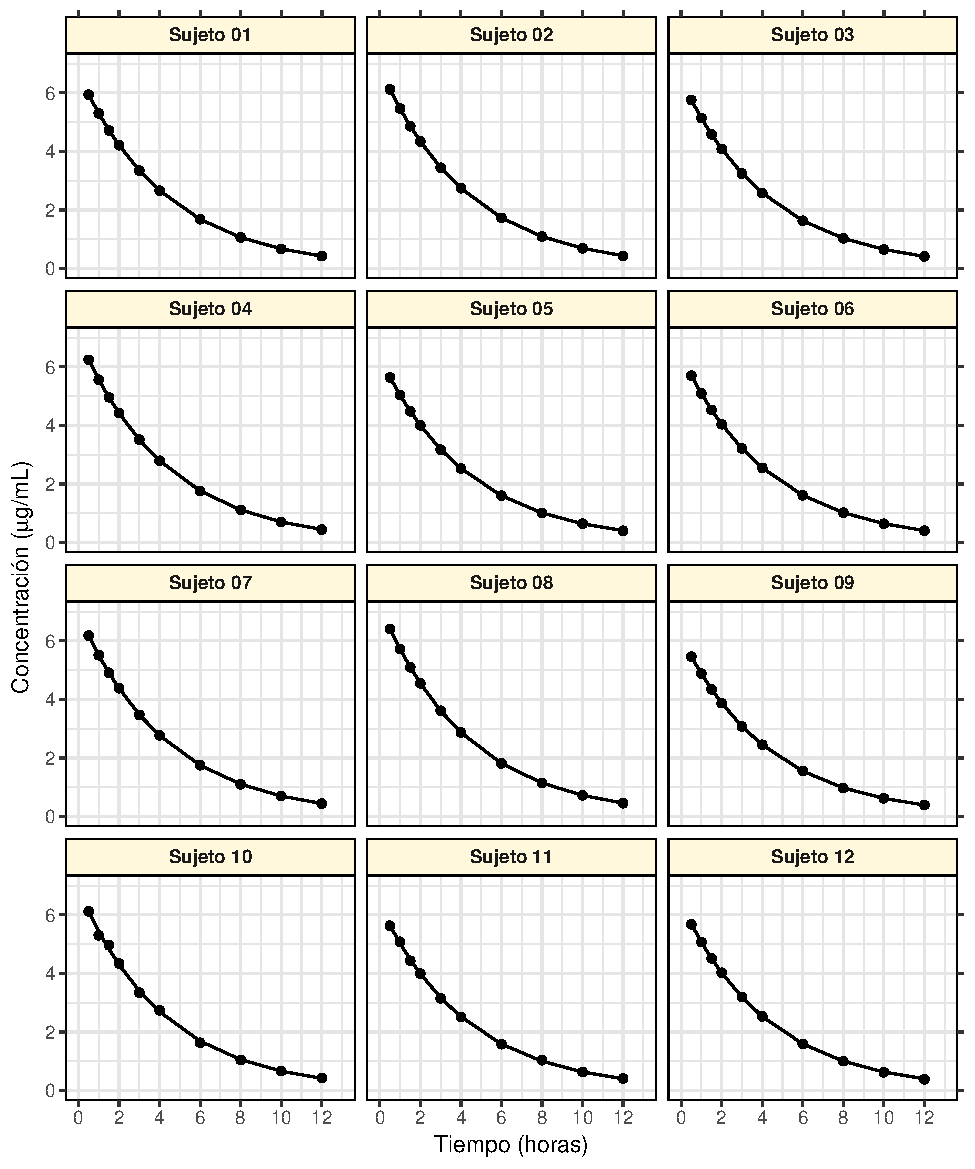
\includegraphics{parcial_1_files/figure-latex/unnamed-chunk-4-1} 

}

\caption{Producto IV - Datos Individuales}\label{fig:unnamed-chunk-4}
\end{figure}

\begin{figure}[H]

{\centering 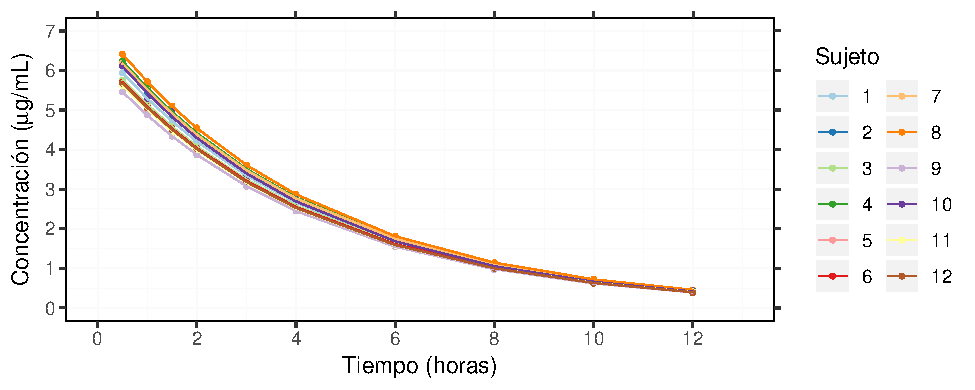
\includegraphics{parcial_1_files/figure-latex/unnamed-chunk-5-1} 

}

\caption{Producto IV - Datos Agrupados}\label{fig:unnamed-chunk-5}
\end{figure}

\begin{figure}[H]

{\centering 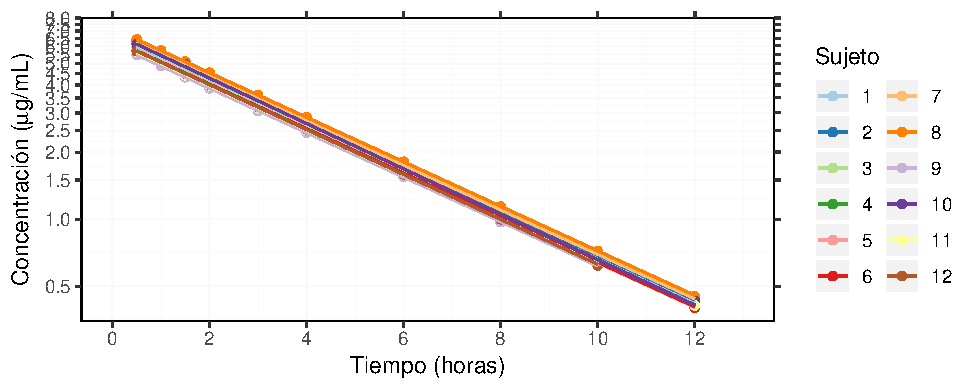
\includegraphics{parcial_1_files/figure-latex/unnamed-chunk-6-1} 

}

\caption{Producto IV - Datos Agrupados (Escala Ln)}\label{fig:unnamed-chunk-6}
\end{figure}

\pagebreak
\pagebreak
\pagebreak
\pagebreak
\pagebreak
\pagebreak
\pagebreak
\pagebreak
\pagebreak
\pagebreak

\subsection{2.2. Modelamiento Individual Datos Administración Producto
A}\label{modelamiento-individual-datos-administracion-producto-a}

En el caso de administración peroral, se tiene en cuenta el modelo con
administración de un bolo en el compartimento de absorción, y se puede
resolver de forma analítica al relacionar \(C_{p}\) y tiempo. Al tener
en cuenta también el error residual, se tiene el siguiente modelo no
lineal:

\[\vec{C_{p}} = \frac{F \cdot D_{0} \cdot k_{a}}{V_{D} \cdot \left(k_{a}-k_{e}\right)}\cdot \left[e^{-k_{e}\cdot\vec{t} }- e^{-k_{a}\cdot\vec{t} } \right] + \vec{\varepsilon} \qquad \varepsilon_{i}\sim \mathcal{N}(0,\,\sigma^{2})\]

En este caso \(F\) es la biodisponibilidad del fármaco para el producto
A, mientras \(k_{a}\) es la constante de velocidad de absorción. El
parámetro \(F\) no se puede resolver sin datos de administración IV por
lo cual se realiza un modelo reducido para el problema de optimización
que tiene en cuenta un volumen de distribución sin el ajuste respectivo
por biodisponibilidad, de la siguiente manera:

\[\vec{C_{p}} = \frac{D_{0} \cdot k_{a}}{V^{*} \cdot \left(k_{a}-k_{e}\right)}\cdot \left[e^{-k_{e}\cdot\vec{t} }- e^{-k_{a}\cdot\vec{t} } \right] + \vec{\varepsilon} \qquad \varepsilon_{i}\sim \mathcal{N}(0,\,\sigma^{2})\]

En este modelo se pueden obtener parámetros farmacocinéticos secundarios
como \(CL_{T}\) y \(t_{1/2}\) de la forma definida previamente. Se hace
un resumen de los diferentes parámetros farmacocinéticos obtenidos para
el producto A en el cuadro 3, recordando que el volumen de distribución
no se ha ajustado a la biodisponibilidad.

\begin{longtable}[]{@{}ccccccc@{}}
\caption{Resultados Parámetros Farmacocinéticos (Producto
A)}\tabularnewline
\toprule
ID & Dosis & \(k_{a}\) & \(k_{e}\) & \(V^{*}\) & \(CL_{T}\) &
\(t_{1/2}\)\tabularnewline
\midrule
\endfirsthead
\toprule
ID & Dosis & \(k_{a}\) & \(k_{e}\) & \(V^{*}\) & \(CL_{T}\) &
\(t_{1/2}\)\tabularnewline
\midrule
\endhead
Sujeto 01 & 700 & 1.504 & 0.23 & 26.279 & 4.788 & 3.017\tabularnewline
Sujeto 02 & 700 & 1.504 & 0.23 & 25.513 & 4.650 & 3.017\tabularnewline
Sujeto 03 & 700 & 1.503 & 0.23 & 27.090 & 4.933 & 3.017\tabularnewline
Sujeto 04 & 700 & 1.503 & 0.23 & 27.653 & 4.564 & 3.015\tabularnewline
Sujeto 05 & 700 & 1.504 & 0.23 & 25.025 & 5.034 & 3.017\tabularnewline
Sujeto 06 & 700 & 1.505 & 0.23 & 24.336 & 4.992 & 3.017\tabularnewline
Sujeto 07 & 700 & 1.503 & 0.23 & 28.559 & 4.599 & 3.017\tabularnewline
Sujeto 08 & 700 & 1.504 & 0.23 & 27.370 & 4.440 & 3.016\tabularnewline
Sujeto 09 & 700 & 1.504 & 0.23 & 25.272 & 5.199 & 3.018\tabularnewline
Sujeto 10 & 700 & 1.501 & 0.23 & 25.510 & 4.732 & 3.008\tabularnewline
Sujeto 11 & 700 & 1.501 & 0.23 & 25.023 & 5.041 & 3.009\tabularnewline
Sujeto 12 & 700 & 1.500 & 0.23 & 25.505 & 5.052 & 3.007\tabularnewline
\bottomrule
\end{longtable}

Para modelos con administración peroral, también se pueden obtener
parámetros biofarmacéuticos como biodisponibilidad absoluta (\(F\)),
concentración plasmática máxima (\(C_{P, max}\)) y tiempo de
\(C_{P, max}\) (\(T_{max}\)). Estos parámetros se definen por las
siguientes fórmulas:

\[F = \frac{\left [ \textrm{AUC}_{\textrm{PO}}\right ]}{\left [ \textrm{AUC}_{\textrm{IV}}\right ]} \times \frac{\left [D_{0}(\textrm{IV})\right ]}{\left [D_{0}(\textrm{PO})\right ]}\]
\[t_{max} = \frac{\ln{k_{a}}-\ln{k_{e}}}{k_{a}-k_{e}}\]

La concentración plasmática máxima se obtiene al reemplazar en la
ecuación analítica el \(t_{max}\). La biodisponibilidad se ha calculado
con datos de \(\textrm{AUC}\) total y truncada. Los resultados en
parámetros biofarmacéuticos se muestran en el cuadro 4 para el producto
A.

\begin{longtable}[]{@{}ccccccc@{}}
\caption{Resultados Parámetros Biofarmacéuticos (Producto
A)}\tabularnewline
\toprule
ID & \(t_{max}\) & \(C_{P,max}\) & AUC\(_{0}^{C_{P}^{*}}\) &
AUC\(_{0}^{\infty}\) & \(F_{AUC_{TRUNC}}\) & \(F_{AUC}\)\tabularnewline
\midrule
\endfirsthead
\toprule
ID & \(t_{max}\) & \(C_{P,max}\) & AUC\(_{0}^{C_{P}^{*}}\) &
AUC\(_{0}^{\infty}\) & \(F_{AUC_{TRUNC}}\) & \(F_{AUC}\)\tabularnewline
\midrule
\endhead
Sujeto 01 & 1.475 & 18.983 & 107.125 & 115.788 & 0.783 &
0.793\tabularnewline
Sujeto 02 & 1.474 & 19.554 & 110.343 & 119.267 & 0.783 &
0.793\tabularnewline
Sujeto 03 & 1.475 & 18.414 & 103.922 & 112.324 & 0.783 &
0.793\tabularnewline
Sujeto 04 & 1.475 & 18.036 & 101.767 & 109.991 & 0.709 &
0.718\tabularnewline
Sujeto 05 & 1.475 & 19.934 & 112.505 & 121.604 & 0.865 &
0.876\tabularnewline
Sujeto 06 & 1.474 & 20.502 & 115.680 & 125.039 & 0.881 &
0.893\tabularnewline
Sujeto 07 & 1.475 & 17.465 & 98.570 & 106.536 & 0.692 &
0.701\tabularnewline
Sujeto 08 & 1.475 & 18.224 & 102.823 & 111.134 & 0.696 &
0.706\tabularnewline
Sujeto 09 & 1.474 & 19.743 & 111.428 & 120.442 & 0.885 &
0.896\tabularnewline
Sujeto 10 & 1.475 & 19.535 & 110.108 & 118.920 & 0.795 &
0.805\tabularnewline
Sujeto 11 & 1.475 & 19.915 & 112.270 & 121.257 & 0.865 &
0.875\tabularnewline
Sujeto 12 & 1.475 & 19.536 & 110.088 & 118.895 & 0.846 &
0.860\tabularnewline
\bottomrule
\end{longtable}

En el cuadro 5 se muestran los parámetros de diagnóstico del modelo,
para los datos del producto A, en general se observa muy buen ajuste del
modelo, por lo cual no se realiza análisis de residuales y pruebas de
suposiciones de regresión.

\begin{longtable}[]{@{}cccc@{}}
\caption{Diagnósticos Modelos (Producto A)}\tabularnewline
\toprule
ID & \(R^{2}\) & \(g_{L}\) & RSE\tabularnewline
\midrule
\endfirsthead
\toprule
ID & \(R^{2}\) & \(g_{L}\) & RSE\tabularnewline
\midrule
\endhead
Sujeto 01 & 0.999997 & 8 & 0.01935\tabularnewline
Sujeto 02 & 0.999997 & 8 & 0.02148\tabularnewline
Sujeto 03 & 0.999997 & 8 & 0.01971\tabularnewline
Sujeto 04 & 0.999997 & 8 & 0.01943\tabularnewline
Sujeto 05 & 0.999997 & 8 & 0.02132\tabularnewline
Sujeto 06 & 0.999997 & 8 & 0.02136\tabularnewline
Sujeto 07 & 0.999997 & 8 & 0.01751\tabularnewline
Sujeto 08 & 0.999997 & 8 & 0.01963\tabularnewline
Sujeto 09 & 0.999997 & 8 & 0.01921\tabularnewline
Sujeto 10 & 0.999996 & 8 & 0.02253\tabularnewline
Sujeto 11 & 0.999996 & 8 & 0.02227\tabularnewline
Sujeto 12 & 0.999996 & 8 & 0.02317\tabularnewline
\bottomrule
\end{longtable}

En la figura 4 se pueden observar los datos observados y curva con
ajuste del modelo discriminado por individuos, etiquetados en
\texttt{azul\ celeste}. En la figura 5 y figura 6 se pueden observar
todos los datos de administración PO (producto A) superpuestos en escala
de concentraciones normal y logarítmica respectivamente.

\begin{figure}[H]

{\centering 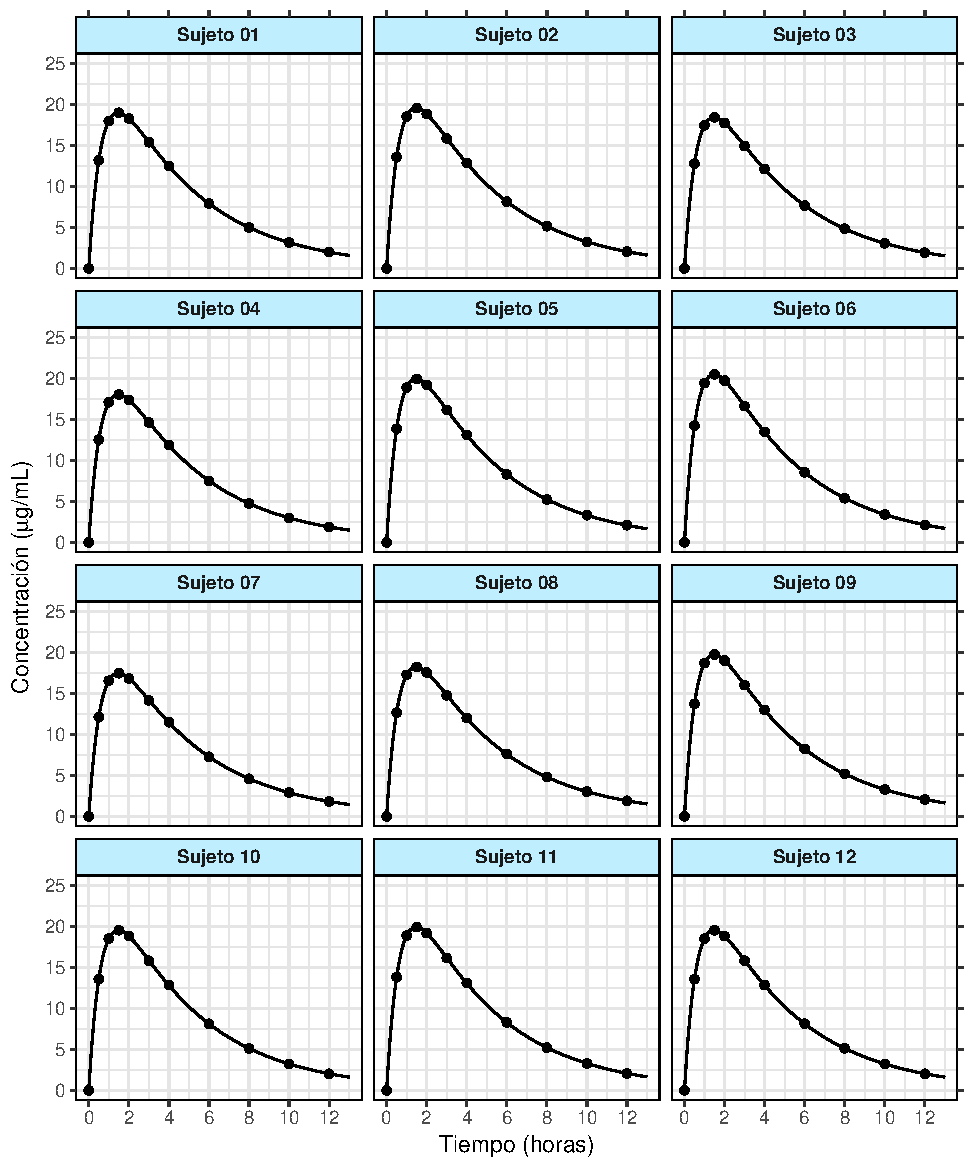
\includegraphics{parcial_1_files/figure-latex/unnamed-chunk-10-1} 

}

\caption{Producto A - Datos Individuales}\label{fig:unnamed-chunk-10}
\end{figure}

\begin{figure}[H]

{\centering 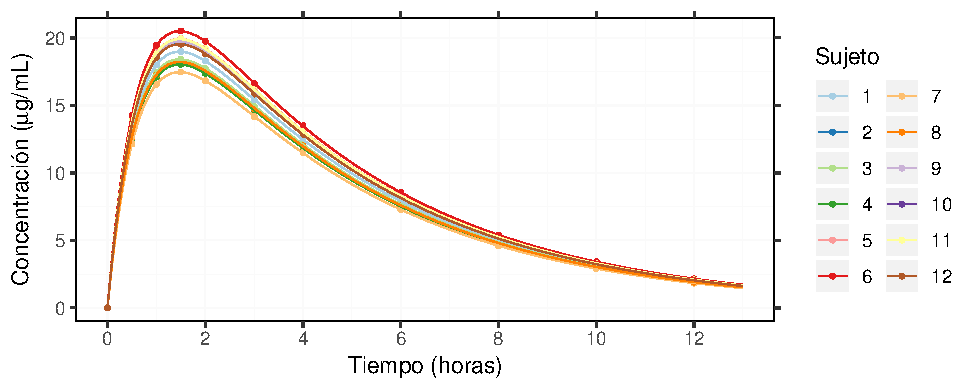
\includegraphics{parcial_1_files/figure-latex/unnamed-chunk-11-1} 

}

\caption{Producto A - Datos Agrupados}\label{fig:unnamed-chunk-11}
\end{figure}

\begin{figure}[H]

{\centering 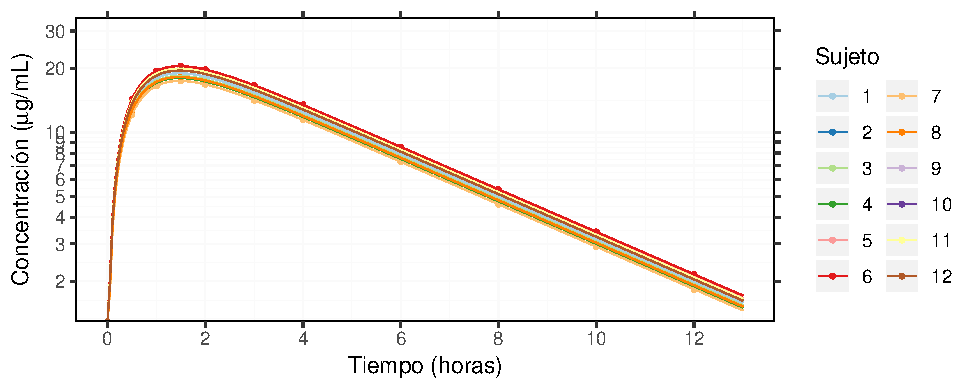
\includegraphics{parcial_1_files/figure-latex/unnamed-chunk-12-1} 

}

\caption{Producto A - Datos Agrupados (Escala Ln)}\label{fig:unnamed-chunk-12}
\end{figure}

\subsection{2.3. Modelamiento Individual Datos Administración Producto
B}\label{modelamiento-individual-datos-administracion-producto-b}

Se hace un resumen de los diferentes parámetros farmacocinéticos
obtenidos para el producto B en el cuadro 6, recordando que el volumen
de distribución no se ha ajustado a la biodisponibilidad.

\begin{longtable}[]{@{}ccccccc@{}}
\caption{Resultados Parámetros Farmacocinéticos (Producto
B)}\tabularnewline
\toprule
ID & Dosis & \(k_{a}\) & \(k_{e}\) & \(V^{*}\) & \(CL_{T}\) &
\(t_{1/2}\)\tabularnewline
\midrule
\endfirsthead
\toprule
ID & Dosis & \(k_{a}\) & \(k_{e}\) & \(V^{*}\) & \(CL_{T}\) &
\(t_{1/2}\)\tabularnewline
\midrule
\endhead
Sujeto 01 & 700 & 2.797 & 0.23 & 26.286 & 4.760 & 3.018\tabularnewline
Sujeto 02 & 700 & 2.797 & 0.23 & 25.276 & 4.624 & 3.018\tabularnewline
Sujeto 03 & 700 & 2.796 & 0.23 & 27.379 & 4.905 & 3.019\tabularnewline
Sujeto 04 & 700 & 2.797 & 0.23 & 28.574 & 4.537 & 3.018\tabularnewline
Sujeto 05 & 700 & 2.796 & 0.23 & 24.334 & 5.005 & 3.017\tabularnewline
Sujeto 06 & 700 & 2.798 & 0.23 & 25.032 & 4.964 & 3.018\tabularnewline
Sujeto 07 & 700 & 2.797 & 0.23 & 27.661 & 4.573 & 3.017\tabularnewline
Sujeto 08 & 700 & 2.796 & 0.23 & 25.519 & 4.414 & 3.018\tabularnewline
Sujeto 09 & 700 & 2.797 & 0.23 & 27.099 & 5.171 & 3.018\tabularnewline
Sujeto 10 & 700 & 2.793 & 0.23 & 25.281 & 4.705 & 3.011\tabularnewline
Sujeto 11 & 700 & 2.792 & 0.23 & 24.340 & 5.011 & 3.011\tabularnewline
Sujeto 12 & 700 & 2.791 & 0.23 & 27.386 & 5.023 & 3.011\tabularnewline
\bottomrule
\end{longtable}

Los resultados en cuanto a parámetros biofarmacéuticos se muestran en el
cuadro 7 para el producto B.

\begin{longtable}[]{@{}ccccccc@{}}
\caption{Resultados Parámetros Biofarmacéuticos (Producto
B)}\tabularnewline
\toprule
ID & \(t_{max}\) & \(C_{P,max}\) & AUC\(_{0}^{C_{P}^{*}}\) &
AUC\(_{0}^{\infty}\) & \(F_{AUC_{TRUNC}}\) & \(F_{AUC}\)\tabularnewline
\midrule
\endfirsthead
\toprule
ID & \(t_{max}\) & \(C_{P,max}\) & AUC\(_{0}^{C_{P}^{*}}\) &
AUC\(_{0}^{\infty}\) & \(F_{AUC_{TRUNC}}\) & \(F_{AUC}\)\tabularnewline
\midrule
\endhead
Sujeto 01 & 0.974 & 21.295 & 107.190 & 115.160 & 0.783 &
0.789\tabularnewline
Sujeto 02 & 0.974 & 22.146 & 111.457 & 119.731 & 0.791 &
0.797\tabularnewline
Sujeto 03 & 0.974 & 20.444 & 102.922 & 110.589 & 0.775 &
0.780\tabularnewline
Sujeto 04 & 0.974 & 19.590 & 98.615 & 105.932 & 0.687 &
0.692\tabularnewline
Sujeto 05 & 0.974 & 23.001 & 115.755 & 124.332 & 0.889 &
0.895\tabularnewline
Sujeto 06 & 0.974 & 22.364 & 112.573 & 120.935 & 0.857 &
0.864\tabularnewline
Sujeto 07 & 0.974 & 20.235 & 101.823 & 109.397 & 0.715 &
0.720\tabularnewline
Sujeto 08 & 0.974 & 21.934 & 110.418 & 118.606 & 0.748 &
0.753\tabularnewline
Sujeto 09 & 0.974 & 20.656 & 103.962 & 111.714 & 0.825 &
0.831\tabularnewline
Sujeto 10 & 0.974 & 22.128 & 111.222 & 119.390 & 0.803 &
0.808\tabularnewline
Sujeto 11 & 0.974 & 22.982 & 115.520 & 123.991 & 0.890 &
0.894\tabularnewline
Sujeto 12 & 0.974 & 20.425 & 102.688 & 110.248 & 0.789 &
0.797\tabularnewline
\bottomrule
\end{longtable}

En el cuadro 8 se muestran los parámetros de diagnóstico del modelo,
para los datos del producto B, en general se observa muy buen ajuste del
modelo, por lo cual no se realiza análisis de residuales y pruebas de
suposiciones de regresión.

\begin{longtable}[]{@{}cccc@{}}
\caption{Diagnósticos Modelos (Producto B)}\tabularnewline
\toprule
ID & \(R^{2}\) & \(g_{L}\) & RSE\tabularnewline
\midrule
\endfirsthead
\toprule
ID & \(R^{2}\) & \(g_{L}\) & RSE\tabularnewline
\midrule
\endhead
Sujeto 01 & 0.999997 & 8 & 0.02052\tabularnewline
Sujeto 02 & 0.999998 & 8 & 0.02076\tabularnewline
Sujeto 03 & 0.999997 & 8 & 0.02065\tabularnewline
Sujeto 04 & 0.999997 & 8 & 0.01957\tabularnewline
Sujeto 05 & 0.999997 & 8 & 0.02299\tabularnewline
Sujeto 06 & 0.999998 & 8 & 0.02104\tabularnewline
Sujeto 07 & 0.999997 & 8 & 0.01952\tabularnewline
Sujeto 08 & 0.999997 & 8 & 0.02206\tabularnewline
Sujeto 09 & 0.999998 & 8 & 0.01931\tabularnewline
Sujeto 10 & 0.999997 & 8 & 0.02331\tabularnewline
Sujeto 11 & 0.999997 & 8 & 0.02575\tabularnewline
Sujeto 12 & 0.999997 & 8 & 0.02315\tabularnewline
\bottomrule
\end{longtable}

En la figura 7 se pueden observar los datos observados y curva con
ajuste del modelo discriminado por individuos, etiquetados en
\texttt{verde}. En la figura 8 y figura 9 se pueden observar todos los
datos de administración PO (producto B) superpuestos en escala de
concentraciones normal y logarítmica respectivamente.

\begin{figure}[H]

{\centering 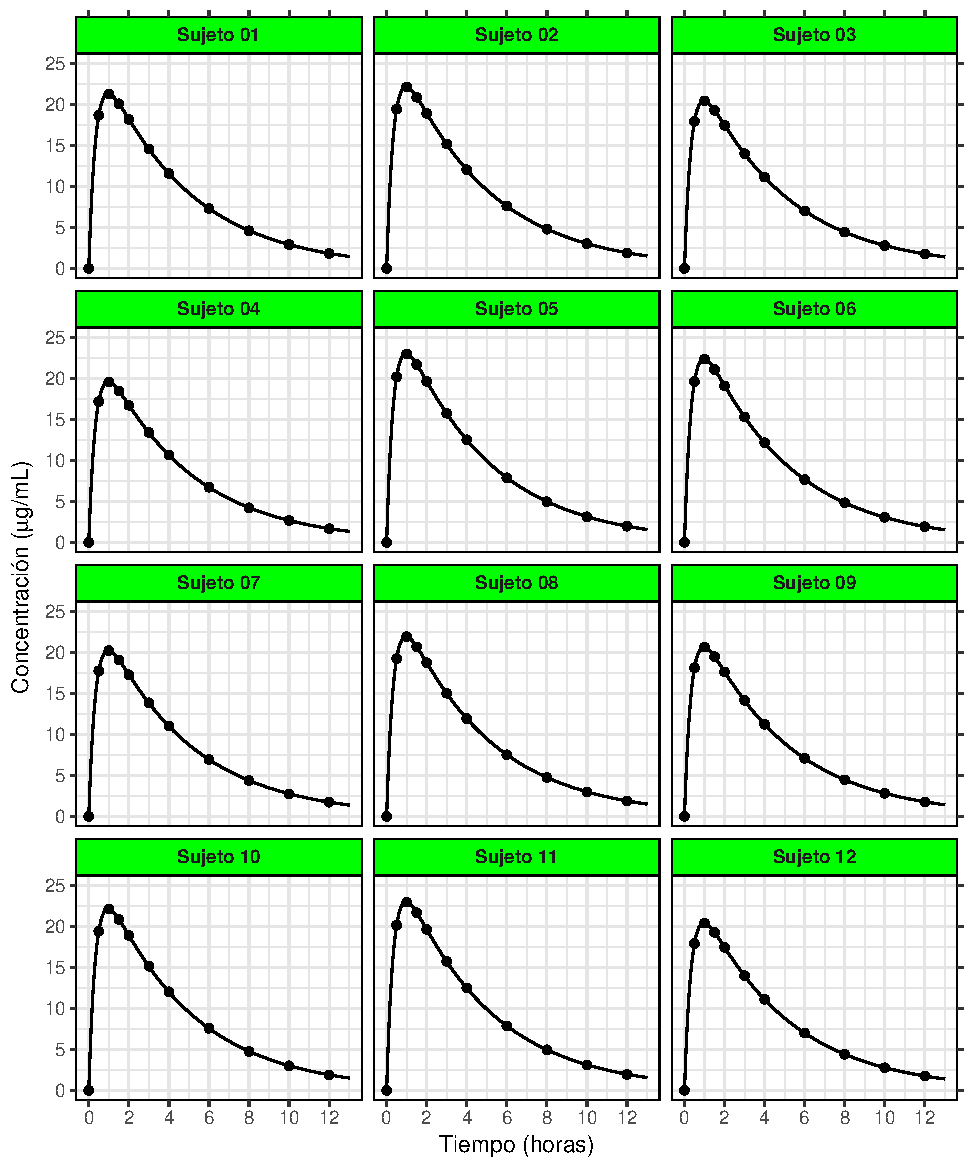
\includegraphics{parcial_1_files/figure-latex/unnamed-chunk-16-1} 

}

\caption{Producto B - Datos Individuales}\label{fig:unnamed-chunk-16}
\end{figure}

\begin{figure}[H]

{\centering 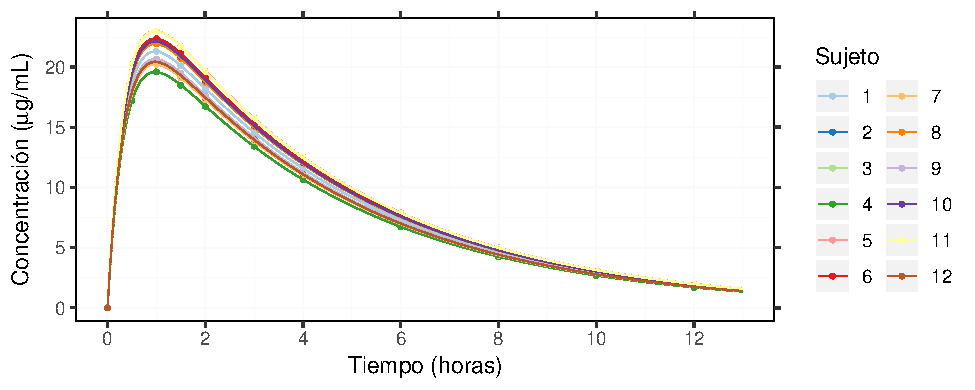
\includegraphics{parcial_1_files/figure-latex/unnamed-chunk-17-1} 

}

\caption{Producto B - Datos Agrupados}\label{fig:unnamed-chunk-17}
\end{figure}

\begin{figure}[H]

{\centering 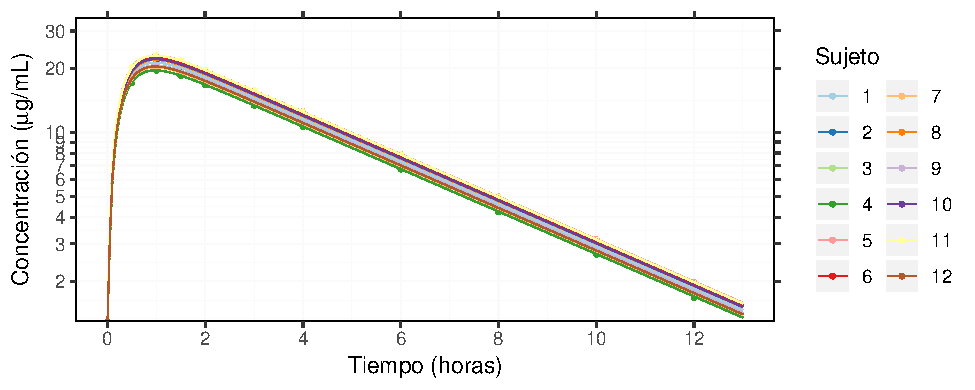
\includegraphics{parcial_1_files/figure-latex/unnamed-chunk-18-1} 

}

\caption{Producto B - Datos Agrupados (Escala Ln)}\label{fig:unnamed-chunk-18}
\end{figure}

\subsection{2.4. Comparación de
Resultados}\label{comparacion-de-resultados}

Los intervalos de confianza de parámetros farmacocinéticos casi siempre
tienen una distribución log-normal. En este caso se ha realizado el test
de Shapiro-Wilk en el conjunto de parámetros para conocer si siguen la
distribución normal. Para \(V_{D}\) (p = 0.058), \(k_{e}\) (p =
8.73E-10), y \(k_{a}\) (p = 1.88E-06), el valor p al ser menor que
\(\alpha\) = 0.05 implica que la distribución de los datos en la muestra
no se adapta a la distribución de los datos de una población normal con
parámetros iguales. En la transformación de logaritmo no se observa
tampoco normalidad, sin embargo, en histogramas se puede observar
log-normalidad en \(k_{e}\), bi-modalidad en \(k_{a}\), y normalidad en
\(V_{D}\).

En los parámetros biofarmacéuticos se tiene que no se puede rechazar la
hipótesis nula de que la muestra proviene de una población con
distribución normal para \(\textrm{AUC}\) (p = 0.431 para A, y p = 0.408
para B), y \(C_{\textrm{MAX}}\) (p = 0.366 para A, y p = 0.377 para B)
al ser transformados a logaritmo natural.

Se realiza el cálculo de intervalos de confianza para cada parámetro por
forma de administración de acuerdo al método de Cox (estimación de media
aritmética en distribuciones log normal)
(\protect\hyperlink{ref-Olsson2005}{1}). Estos intervalos son definidos
por la siguiente fórmula:

\[\bar{Y} + \frac{\sigma^{2}}{2} \pm \left [ t_{1-\frac{\alpha}{2},g_{L}} \cdot \sqrt{\frac{\sigma^{2}}{n} + \frac{\sigma^{4}}{2(n-1)}} \right]\]

En donde, \(\bar{Y}\) y \(\sigma^{2}\) son la media aritmética y
varianza de los valores log-transformados, estos valores se vuelven a
transformar por exponenciación. El promedio en este método de estimación
sigue la fórmula \(\hat{\theta} = e^{\bar{Y}+\frac{S^{2}}{2}}\). En los
cuadro 9 y 10 se puede observar una comparación entre productos,
teniendo en cuenta el promedo aritmético de los datos originales, e
intervalos de confianza (de Cox) de parámetros farmacocinéticos y
biofarmacéuticos.

\begin{longtable}[]{@{}lcrcrcr@{}}
\caption{Comparación Parámetros Farmacocinéticos}\tabularnewline
\toprule
& Producto IV & IC 95\% & Producto A & IC 95\% & Producto B & IC
95\%\tabularnewline
\midrule
\endfirsthead
\toprule
& Producto IV & IC 95\% & Producto A & IC 95\% & Producto B & IC
95\%\tabularnewline
\midrule
\endhead
\(V_{D}\) & 21.16 & 20.472 - 21.83 & 21.03 & 20.358 - 21.681 & 20.92 &
20.254 - 21.569\tabularnewline
\(k_{e}\) & 0.23 & 0.23 - 0.231 & 0.23 & 0.23 - 0.23 & 0.23 & 0.23 -
0.23\tabularnewline
\(CL_{T}\) & 4.88 & 4.719 - 5.029 & 4.84 & 4.68 - 4.985 & 4.81 & 4.653 -
4.956\tabularnewline
\(t_{1/2}\) & 3.01 & 2.996 - 3.019 & 3.01 & 3.012 - 3.017 & 3.02 & 3.014
- 3.018\tabularnewline
\(k_{a}\) & - & - & 1.50 & 1.502 - 1.504 & 2.80 & 2.794 -
2.797\tabularnewline
\(\textrm{AUC}_{\textrm{trunc}}\) & 27.17 & 26.292 - 28.009 & 108.05 &
104.657 - 111.319 & 107.85 & 104.106 - 111.428\tabularnewline
\(\textrm{AUC}\) & 28.98 & 28.042 - 29.873 & 116.77 & 113.104 - 120.29 &
115.84 & 111.831 - 119.672\tabularnewline
\bottomrule
\end{longtable}

\begin{longtable}[]{@{}lcrcr@{}}
\caption{Comparación Parámetros Biofarmacéuticos}\tabularnewline
\toprule
& Producto A & IC 95\% & Producto B & IC 95\%\tabularnewline
\midrule
\endfirsthead
\toprule
& Producto A & IC 95\% & Producto B & IC 95\%\tabularnewline
\midrule
\endhead
\(t_{max}\) & 1.475 & 1.47455 - 1.47501 & 0.974 & 0.97368 -
0.97404\tabularnewline
\(C_{max}\) & 19.153 & 18.5495 - 19.73442 & 21.433 & 20.68773 -
22.14738\tabularnewline
\(F_{\textrm{trunc}}\) & 0.798 & 0.7508 - 0.84285 & 0.796 & 0.75449 -
0.83513\tabularnewline
\(F_{\textrm{total}}\) & 0.809 & 0.76074 - 0.85396 & 0.802 & 0.76 -
0.84084\tabularnewline
\bottomrule
\end{longtable}

\section{3. Inferencias Estadísticas para
Efectos}\label{inferencias-estadisticas-para-efectos}

\subsection{3.1. Enunciado del Problema}\label{enunciado-del-problema}

En el presente estudio se tiene un diseño cruzado 2 x 2 estándar que
puede ser analizado por medio de pruebas estadísticas basadas en dos
muestras (no pareadas). En el enunciado inicial del problema no se
identifica el grupo (secuencia) de tratamiento de cada individuo, por lo
cual se realiza un muestreo aleatorio sin reemplazo de las siguientes
secuencias de tratamiento:

\begin{longtable}[]{@{}ccc@{}}
\caption{Grupos o Secuencias de Tratamiento}\tabularnewline
\toprule
Secuencia & Periodo 1 & Periodo 2\tabularnewline
\midrule
\endfirsthead
\toprule
Secuencia & Periodo 1 & Periodo 2\tabularnewline
\midrule
\endhead
1 (RC) & Formulación Referencia (\(Y_{i11}\)) & Formulación Competidor
(\(Y_{i21}\))\tabularnewline
2 (CR) & Formulación Competidor (\(Y_{i12}\)) & Formulación Referencia
(\(Y_{i21}\))\tabularnewline
\bottomrule
\end{longtable}

\begin{longtable}[]{@{}cccccc@{}}
\caption{Asignación a Secuencias de Tratamiento}\tabularnewline
\toprule
Sujeto & Secuencia & Sujeto & Secuencia & Sujeto &
Secuencia\tabularnewline
\midrule
\endfirsthead
\toprule
Sujeto & Secuencia & Sujeto & Secuencia & Sujeto &
Secuencia\tabularnewline
\midrule
\endhead
1 & 2 (TR) & 5 & 1 (RT) & 9 & 1 (RT)\tabularnewline
2 & 1 (RT) & 6 & 2 (TR) & 10 & 2 (TR)\tabularnewline
3 & 2 (TR) & 7 & 2 (TR) & 11 & 1 (RT)\tabularnewline
4 & 1 (RT) & 8 & 2 (TR) & 12 & 1 (RT)\tabularnewline
\bottomrule
\end{longtable}

\subsection{3.2. Introducción al modelo
general}\label{introduccion-al-modelo-general}

\subsubsection{3.2.1. Modelo General}\label{modelo-general}

\begin{quote}
Los métodos y modelos estadísticos de análisis, descritos en el presente
documento son tomados de Chow Shein y colaboradores
(\protect\hyperlink{ref-Chow2009}{2}) capítulos 1, 3, 4, y 6.
\end{quote}

El modelo general que describe al diseño cruzado 2x2, para el
\(i \textrm{(sujeto)} = 1,2,\cdots,n_{k}\),
\(j \textrm{(periodo),} k\textrm{(secuencia) = 1,2}\) es el siguiente:
\[Y_{ijk} = \mu + S_{ik} + P_{j} + F_{(j,k)}+C_{j-1,k}+e_{ijk}\]

En donde, \(Y_{ijk}\) es la observación (que puede ser \(\ln{C_{max}}\)
o \(\ln{\textrm{AUC}}\)) definida para el i-ésimo sujeto, en el j-ésimo
periodo y k-ésima secuencia, \(\mu\) es la media general de las
observaciones, \(S_{ik}\) es el efecto aleatorio del i-ésimo sujeto en
la k-ésima secuencia, \(P{j}\) es el efecto fijo del j-ésimo periodo,
\(F_{j,k}\) es el efecto fijo directo de la formulación en la k-ésima
secuencia y j-ésimo periodo, \(C{j-1,k}\) es el efecto fijo de efecto de
\emph{carry-over} de primer órden de la formulación en la k-ésima
secuencia y (j-1)-ésimo periodo, y por último, \(e_{ijk}\) es el error
aleatorio (intra individual) en el \(Y_{ijk}\).

Se deben cumplir varias suposiciones como \(\sum_{j}{P_{j}}\),
\(\sum{F_{j,k}}\), \(\sum{C_{0,k}}\), y \(\sum{C_{(j-1,k)}}\) son todos
iguales a cero, \(S_{i,k}\) se encuentra \(i.i.d.\) con media 0 y
varianza \(\sigma^{2}_{S}\), mientras los \(e_{ijk}\) tienen media 0 y
varianza \(\sigma_{t}^{2}\). El modelo tiene en cuenta variabilidad
inter- e intra-individual. En adición, se debe cumplir que:

\[F_{j,k} = \left\{\begin{matrix} F_{R} \textrm{ si } k=j \\ F_{T} \textrm{ si } k \neq j \end{matrix}\right.\]
Por la misma definición de las secuencias si se considera el periodo 1 y
secuencia 1 se tiene el efecto de la formulación de referencia. En
adición, se considera el efecto de \emph{carry-over}:

\[C_{j-1,k} = \left\{\begin{matrix} C_{R} \textrm{ si } k = 1, j =2 \\ C_{T} \textrm{ si } k = 2, j =2 \end{matrix}\right.\]
Este efecto es debido a la administración de una dosis anterior en el
primer periodo para el segundo, y se puede dar cuando no hay un buen
periodo de lavado. La significancia de los diferentes efectos puede ser
estimada por medio de diferentes ecuaciones. Debido a que se realiza una
transformación logarítmica debe tenerse en cuenta que para los
parámetros originales el modelo es multiplicativo:
\[X_{ijk} = e^{Y_{ijk}} = \tilde{\mu}\tilde{S}_{ik}\tilde{P}_{j}\tilde{F}_{(j,k)}\tilde{C}_{j-1,k}\tilde{e}_{ijk}\]

\subsubsection{\texorpdfstring{3.2.2. Efecto de
\emph{Carry-Over}}{3.2.2. Efecto de Carry-Over}}\label{efecto-de-carry-over}

Su estimador \(\hat{C}\) se calcula teniendo en cuenta los totales por
sujeto para cada secuencia:
\[\hat{C} = \bar{U}_{\bullet2} - \bar{U}_{\bullet1}\] Estos totales se
calculan de la siguiente manera:\\
\[U_{ij} = Y_{i1k}+Y_{i2k}\] En este caso se suma las observaciones de
cada sujeto en cada secuencia, estas se promedian en la secuencia k para
obtener \(\bar{U}_{\bullet k}\). La varianza estimada
\(\hat{V}(\hat{C})\), se describe por las siguientes ecuaciones:
\[\hat{V}(\hat{C}) = \sigma_{u}^{2}\left (\frac{1}{n_{1}}+\frac{1}{n_{2}} \right )\]
\[\hat{\sigma_{u}^{2}} = \frac{1}{n_{1}+n_{2}-2} \sum_{k=1}^{2}\sum_{i=1}^{n_{k}}{(U_{ik}-\bar{U}_{\bullet k})^{2}}\]
Se utiliza una prueba t (no pareada) para conocer la ``significancia''
de este efecto, es decir, si es diferente de cero. El \(T_{\textrm{c}}\)
y el intervalo de confianza se calculan por medio de las siguientes
ecuaciones:\\
\[T_{\textrm{c}} = \frac{\hat{C}}{\hat{\sigma_{u}}\cdot\sqrt{\frac{1}{n_{1}}+\frac{1}{n_{2}}}}\]
\[\hat{C} \pm t_{\alpha/2, n_{1}+n_{2}-2} \hat{\sigma_{u}} \sqrt{\frac{1}{n_{1}}+\frac{1}{n_{2}}}\]

Las hipótesis son las siguientes \(H_{0}: C=0\) o \((C_{R} = C_{C})\) vs
\(H_{a}: C \neq 0\) o \((C_{R} \neq C_{C})\). Si se cumple \(H_{0}\) se
tiene que \(T_{\textrm{c}}\) tiene una distribución central t con
\(g_{L} = n_{1}+n_{2}-2\), por tal, se rechaza la \(H_{0}\) si:\\
\[\left |T_{\textrm{c}} \right | > t_{\alpha/2,n_{1}+n_{2}-2}\]

\subsubsection{\texorpdfstring{3.2.3. Efecto de
\emph{Formulación}}{3.2.3. Efecto de Formulación}}\label{efecto-de-formulacion}

Se deben definir inicialmente las diferencias en el valor observado del
periodo 2 al periodo 1 en cada sujeto y en cada secuencia:\\
\[d_{ik} = \frac{1}{2} \left ( Y_{i2k} -Y_{i1k}\right ),\textrm{ para }i=1,2,...,n_{k}; k = 1,2\]
Se distinguen dos casos, cuando \(C_{R}=C_{C}\) (no \emph{carry-over}) y
\(C_{R} \neq C_{C}\) (hay \emph{carry-over}), en el segundo caso no es
posible obtener estimadores no sesgados del efecto de la formulación. En
el caso sin carry-over se define al estimador del efecto de la
formulación como:

\[\hat{F} = \bar{d}_{\bullet1}-\bar{d}_{\bullet2}\]
\[\hat{F} = \frac{1}{2}\left[\left(\bar{Y}_{\bullet21}-\bar{Y}_{\bullet11}\right)-\left(\bar{Y}_{\bullet22}-\bar{Y}_{\bullet12}\right)\right]\]
\[\hat{F} = \bar{Y}_{C}-\bar{Y}_{R}\] De manera alternativa, se puede
obtener el estimador por medio de la siguiente fórmula:\\
\[\hat{F}^{*} = \frac{1}{n_{1}+n_{2}} \cdot\left(\left\{\sum_{i=1}^{n_{1}}{Y_{i21}}+\sum_{i=1}^{n_{2}}{Y_{i12}}\right\}-\left\{\sum_{i=1}^{n_{1}}{Y_{i11}}+\sum_{i=1}^{n_{2}}{Y_{i22}}\right\}\right )\]
La varianza del estimador se puede obtener por medio de las siguientes
fórmulas:

\[\hat{V}(\hat{F}) = \sigma_{d}^{2}\left (\frac{1}{n_{1}}+\frac{1}{n_{2}} \right )\]
\[\hat{\sigma_{d}^{2}} = \frac{1}{n_{1}+n_{2}-2} \sum_{k=1}^{2}\sum_{i=1}^{n_{k}}{(d_{ik}-\bar{d}_{\bullet k})^{2}}\]
Se utiliza una prueba t (no pareada) para conocer la ``significancia''
de este efecto, es decir, si es diferente de cero. El \(T_{\textrm{d}}\)
y el intervalo de confianza se calculan por medio de las siguientes
ecuaciones:\\
\[T_{\textrm{d}} = \frac{\hat{F}}{\hat{\sigma_{d}}\cdot\sqrt{\frac{1}{n_{1}}+\frac{1}{n_{2}}}}\]
\[\hat{F} \pm t_{\alpha/2, n_{1}+n_{2}-2} \hat{\sigma_{d}} \sqrt{\frac{1}{n_{1}}+\frac{1}{n_{2}}}\]
Las hipótesis son las siguientes \(H_{0}: F=0\) o \((F_{R} = F_{C})\) vs
\(H_{a}: F \neq 0\) o \((F_{R} \neq F_{C})\). Si se cumple \(H_{0}\) se
tiene que \(T_{\textrm{d}}\) tiene una distribución central t con
\(g_{L} = n_{1}+n_{2}-2\), por tal, se rechaza la \(H_{0}\) si:\\
\[\left |T_{\textrm{d}} \right | > t_{\alpha/2,n_{1}+n_{2}-2}\]

\subsubsection{\texorpdfstring{3.2.4. Efecto de Formulación (cuando hay
\emph{carry-over})}{3.2.4. Efecto de Formulación (cuando hay carry-over)}}\label{efecto-de-formulacion-cuando-hay-carry-over}

Se puede obtener un estimador no sesgado de \(F\) si sólo se utilizan
los datos del primer periodo para cada sujeto, sin embargo, se pierden
datos y precisión en la estimación. El estimador y su varianza se pueden
calcular por medio de las siguientes expresiones:\\
\[\hat{F}|C = \bar{Y}_{\bullet12} - \bar{Y}_{\bullet11}\]
\[V(\hat{F}|C) = (\sigma_{S}^{2}+\sigma_{e}^{2})\left (\frac{1}{n_{1}}+\frac{1}{n_{2}}\right)\]
En la práctica, es de importancia extrema tener un periodo de lavado
suficiente entre periodos de dosificación para eliminar efectos de
administración previa. El estimados no sesgado de la varianza es el
siguiente:\\
\[\hat{V}(\hat{F}|C) = (S_{f}^{2})\left (\frac{1}{n_{1}}+\frac{1}{n_{2}}\right)\]
\[S_{f}^{2} = \frac{1}{n_{1}+n_{2}-2} \sum_{k=1}^{2}\sum_{i=1}^{n_{k}}{\left ( Y_{i1k} - \bar{Y}_{\bullet1k}\right )^{2}}\]
Se utiliza una prueba t (no pareada) para conocer la ``significancia''
de este efecto, es decir, si es diferente de cero. El \(T_{\textrm{d}}\)
y el intervalo de confianza se calculan por medio de las siguientes
ecuaciones:\\
\[T_{\textrm{d}} = \frac{\hat{F}|C}{S_{f}\cdot\sqrt{\frac{1}{n_{1}}+\frac{1}{n_{2}}}}\]
\[\hat{F}|C \pm t_{\alpha/2, n_{1}+n_{2}-2} S_{f} \sqrt{\frac{1}{n_{1}}+\frac{1}{n_{2}}}\]
Las hipótesis son las siguientes \(H_{0}: F=0\) o \((F_{R} = F_{C})\) vs
\(H_{a}: F \neq 0\) o \((F_{R} \neq F_{C})\). Si se cumple \(H_{0}\) se
tiene que \(T_{\textrm{d}}\) tiene una distribución central t con
\(g_{L} = n_{1}+n_{2}-2\), por tal, se rechaza la \(H_{0}\) si:\\
\[\left |T_{\textrm{d}} \right | > t_{\alpha/2,n_{1}+n_{2}-2}\]\\
Esta forma de análisis con \emph{carry-over} tiene menos poder para
detectar diferencias de bioequivalencia debido a que puede haber mayor
variabilidad inter-individual, en adición hay un sacrificio de la mitad
de la información que elimina los beneficios de un diseño cruzado.

\subsubsection{3.2.5. Efecto del Periodo}\label{efecto-del-periodo}

En cuanto al efecto del periodo se debe considerar como:\\
\[O_{ik} = \left\{\begin{matrix} d_{ik} \textrm{ para sujetos en S1}\\ -d_{ik}\textrm{ para sujetos en S2} \end{matrix}\right.\]
\[\bar{O}_{ik} = \left\{\begin{matrix} \bar{d}_{\bullet1} \textrm{ para k = 1}\\ -\bar{d}_{\bullet2}\textrm{ para k = 2} \end{matrix}\right.\]

El estimador del efecto del periodo se calcula mediante la siguiente
expresión:

\[\hat{P} = \bar{O}_{\bullet1}-\bar{O}_{\bullet2}\] Se utiliza una
prueba t (no pareada) para conocer la ``significancia'' de este efecto,
es decir, si es diferente de cero. El \(T_{\textrm{O}}\) y el intervalo
de confianza se calculan por medio de las siguientes ecuaciones:\\
\[T_{\textrm{O}} = \frac{\hat{P}}{\sigma_{d}^{2}\cdot\sqrt{\frac{1}{n_{1}}+\frac{1}{n_{2}}}}\]
\[\hat{P} \pm t_{\alpha/2, n_{1}+n_{2}-2} \sigma_{d}^{2} \sqrt{\frac{1}{n_{1}}+\frac{1}{n_{2}}}\]
Las hipótesis son las siguientes \(H_{0}: P_{1} = P_{2}\) vs
\(H_{a}: P_{1} \neq P_{2}\). Si se cumple \(H_{0}\) se tiene que
\(T_{\textrm{O}}\) tiene una distribución central t con
\(g_{L} = n_{1}+n_{2}-2\), por tal, se rechaza la \(H_{0}\) si:\\
\[\left |T_{\textrm{O}} \right | > t_{\alpha/2,n_{1}+n_{2}-2}\]

\subsection{3.3. Resultados de Inferencia de efectos en
AUC}\label{resultados-de-inferencia-de-efectos-en-auc}

Para conocer la influencia de los efectos se tiene que hacer
transformación logarítmica de los resultados AUC. Se realizaron los
cálculos previamentes expuestos.

\subsubsection{3.3.1. Carry-Over en AUC}\label{carry-over-en-auc}

Se tiene que \(\bar{U}_{\bullet1}\)=9.527, \(\bar{U}_{\bullet2}\)=9.493,
y \(\hat{\sigma}_{u}^{2}\)=9.15E-03, el valor calculado de t es dado
por:

\[T_{c}=\frac{9.493-9.527}{\sqrt{9.15*10^{-3}}\left(\frac{1}{6}+\frac{1}{6}\right)}=-0.6028\]

Debido a que \(\left|T_{c}\right|=0.6028<t_{0.025,10}\)=2.228, no se
rechaza la hipótesis nula y este efecto no tiene significancia (al no
ser diferente de cero), el valor p de este test es 0.560. El valor
estimado de \emph{carry-over} es
\(\hat{C}=-0.0333\;(\textrm{IC95}\%-0.1563,0.0898)\), el intervalo de
confianza cruza por el valor de cero, lo cual es consistente con el
resultado del test t. Por todo esto, se pueden usar los datos de ambos
periodos para conocer el efecto de la formulación.

\subsubsection{3.3.2. Efecto de Formulación en
AUC}\label{efecto-de-formulacion-en-auc}

Se tiene que \(\bar{d}_{\bullet1}\)=-0.0233,
\(\bar{d}_{\bullet2}\)=-0.0069, y \(\hat{\sigma}_{d}^{2}\)=1.657E-03. El
valor de F es calculado como:
\[\hat{F} = \bar{d}_{\bullet1} - \bar{d}_{\bullet2} = -0.0233 + 0.0069 = -0.0165\]
El cálculo del valor t es dado por:

\[T_{d}=\frac{-0.0165}{\sqrt{1.657*10^{-3}}\left(\frac{1}{6}+\frac{1}{6}\right)}=-0.701\]

Debido a que \(\left|T_{d}\right|=0.701<t_{0.025,10}\)=2.228, no se
rechaza la hipótesis nula y este efecto no tiene significancia (al no
ser diferente de cero), el valor p de este test es 0.4994. El intervalo
de confianza del efecto de formulación es
\(\textrm{IC95}\%-0.0688,0.0359\), este cruza el valor de cero, lo que
es consistente con el resultado del test t. En adición, existe una forma
alternativa de estimar el efecto de formulación bajo la cual
\(\hat{F}=-0.0082\;(\textrm{IC95}\%-0.0606,0.0441)\), en este caso
\(T_{d}\)=-0.3503. Estos resultados indican que el efecto de la
formulación no es significativo en el resultado de AUC.

\subsubsection{3.3.3. Efecto de Periodo en
AUC}\label{efecto-de-periodo-en-auc}

Se tiene que \(\bar{O}_{\bullet1}\)=-0.0233, y
\(\bar{O}_{\bullet2}\)=0.0069, el valor calculado de t es dado por:

\[T_{o}=\frac{0.0069-0.0233}{\sqrt{1.657*10^{-3}}\left(\frac{1}{6}+\frac{1}{6}\right)}=-1.2845\]

Debido a que \(\left|T_{o}\right|=1.2845<t_{0.025,10}\)=2.228, no se
rechaza la hipótesis nula y este efecto no tiene significancia (al no
ser diferente de cero), el valor p de este test es 0.2279. El efecto del
periodo estimado es
\(\hat{P}=-0.0302\;(\textrm{IC95}\%-0.0825,0.0222)\), el intervalo de
confianza cruza por el valor de cero, lo cual es consistente con el
resultado del test t. El efecto del periodo no es significativo en el
valor de AUC.

\subsubsection{3.3.4 Resumen para AUC}\label{resumen-para-auc}

\begin{longtable}[]{@{}lcccc@{}}
\caption{Resultados Inferencia AUC}\tabularnewline
\toprule
& MVUE & IC95\% & T & Valor p\tabularnewline
\midrule
\endfirsthead
\toprule
& MVUE & IC95\% & T & Valor p\tabularnewline
\midrule
\endhead
Carry-Over & -0.0333 & (-0.1563,0.0898) & -0.6028 &
5.601e-01\tabularnewline
Formulación 1 & -0.0165 & (-0.0688,0.0359) & -0.7008 &
4.994e-01\tabularnewline
Formulación 2 & -0.0082 & (-0.0606,0.0441) & -0.3504 &
7.333e-01\tabularnewline
Periodo & -0.0302 & (-0.0825,0.0222) & -1.2845 &
2.279e-01\tabularnewline
\bottomrule
\end{longtable}

\subsection{\texorpdfstring{3.4. Resultados de Inferencia de efectos en
\(C_{max}\)}{3.4. Resultados de Inferencia de efectos en C\_\{max\}}}\label{resultados-de-inferencia-de-efectos-en-c_max}

Para conocer la influencia de los efectos se tiene que hacer
transformación logarítmica de los resultados \(C_{max}\). Se realizaron
los cálculos previamentes expuestos.

\subsubsection{\texorpdfstring{3.4.1. Carry-Over en
\(C_{max}\)}{3.4.1. Carry-Over en C\_\{max\}}}\label{carry-over-en-c_max}

Se tiene que \(\bar{U}_{\bullet1}\)=6.032, \(\bar{U}_{\bullet2}\)=5.998,
y \(\hat{\sigma}_{u}^{2}\)=9.25E-03, el valor calculado de t es dado
por:

\[T_{c}=\frac{5.998-6.032}{\sqrt{9.25*10^{-3}}\left(\frac{1}{6}+\frac{1}{6}\right)}=-0.6124\]

Debido a que \(\left|T_{c}\right|=0.612<t_{0.025,10}\)=2.228, no se
rechaza la hipótesis nula y este efecto no tiene significancia (al no
ser diferente de cero), el valor p de este test es 0.554. El valor
estimado de \emph{carry-over} es
\(\hat{C}=-0.034\;(\textrm{IC95}\%-0.158,0.090)\), el intervalo de
confianza cruza por el valor de cero, lo cual es consistente con el
resultado del test t. Por todo esto, se pueden usar los datos de ambos
periodos para conocer el efecto de la formulación.

\subsubsection{\texorpdfstring{3.4.2. Efecto de Formulación en
\(C_{max}\)}{3.4.2. Efecto de Formulación en C\_\{max\}}}\label{efecto-de-formulacion-en-c_max}

Se tiene que \(\bar{d}_{\bullet1}\)=0.0972,
\(\bar{d}_{\bullet2}\)=-0.1273, y \(\hat{\sigma}_{d}^{2}\)=1.667E-03. El
valor de F es calculado como:
\[\hat{F} = \bar{d}_{\bullet1} - \bar{d}_{\bullet2} = 0.0972 + (-0.1273) = 0.2245\]
El cálculo del valor t es dado por:

\[T_{d}=\frac{0.2245}{\sqrt{1.667*10^{-3}}\left(\frac{1}{6}+\frac{1}{6}\right)}=9.506\]

Debido a que \(\left|T_{d}\right|=9.506>t_{0.025,10}\)=2.228, se rechaza
la hipótesis nula y este efecto tiene significancia, el valor p de este
test es 2.524E-6. El intervalo de confianza del efecto de formulación es
\(\textrm{IC95}\%0.172,0.277\), este intervalo no cruza el cero, lo que
es consistente con el resultado del test t.

De acuerdo a la forma alternativa de estimar el efecto de formulación
bajo la cual \(\hat{F}=0.112\;(\textrm{IC95}\%0.060,0.165)\), en este
caso \(T_{d}\)=4.753 (p = 7.77E-04). Estos resultados indican que existe
un efecto de la formulación en el resultado de \(C_{max}\), por lo cual
no se podría declarar bioequivalencia.

\subsubsection{\texorpdfstring{3.4.3. Efecto de Periodo en
\(C_{max}\)}{3.4.3. Efecto de Periodo en C\_\{max\}}}\label{efecto-de-periodo-en-c_max}

Se tiene que \(\bar{O}_{\bullet1}\)=0.0972, y
\(\bar{O}_{\bullet2}\)=0.1273, el valor calculado de t es dado por:

\[T_{o}=\frac{0.0972-0.1273}{\sqrt{1.667*10^{-3}}\left(\frac{1}{6}+\frac{1}{6}\right)}=-1.273\]

Debido a que \(\left|T_{o}\right|=1.273<t_{0.025,10}\)=2.228, no se
rechaza la hipótesis nula y este efecto no tiene significancia (al no
ser diferente de cero), el valor p de este test es 0.2318. El efecto del
periodo estimado es
\(\hat{P}=-0.0301\;(\textrm{IC95}\%-0.0827,0.0226)\), el intervalo de
confianza cruza por el valor de cero, lo cual es consistente con el
resultado del test t. El efecto del periodo no es significativo en el
valor de \(C_{max}\).

\subsubsection{\texorpdfstring{3.4.4. Resumen para
\(C_{max}\)}{3.4.4. Resumen para C\_\{max\}}}\label{resumen-para-c_max}

\begin{longtable}[]{@{}lcccc@{}}
\caption{Resultados Inferencia \(C_{max}\)}\tabularnewline
\toprule
& MVUE & IC95\% & T & Valor p\tabularnewline
\midrule
\endfirsthead
\toprule
& MVUE & IC95\% & T & Valor p\tabularnewline
\midrule
\endhead
Carry-Over & -0.0340 & (-0.1577,0.0897) & -0.6124 &
5.539e-01\tabularnewline
Formulación 1 & 0.2245 & (0.1718,0.2771) & 9.5059 &
2.524e-06\tabularnewline
Formulación 2 & 0.1122 & (0.0596,0.1648) & 4.7530 &
7.767e-04\tabularnewline
Periodo & -0.0301 & (-0.0827,0.0226) & -1.2730 &
2.318e-01\tabularnewline
\bottomrule
\end{longtable}

\subsection{\texorpdfstring{3.5 Resumen para
\(F_{\textrm{TOTAL}}\)}{3.5 Resumen para F\_\{\textbackslash{}textrm\{TOTAL\}\}}}\label{resumen-para-f_textrmtotal}

\begin{longtable}[]{@{}lcccc@{}}
\caption{Resultados Inferencia \(F_{\textrm{TOTAL}}\)}\tabularnewline
\toprule
& MVUE & IC95\% & T & Valor p\tabularnewline
\midrule
\endfirsthead
\toprule
& MVUE & IC95\% & T & Valor p\tabularnewline
\midrule
\endhead
Carry-Over & -0.1056 & (-0.3159,0.1047) & -1.1190 &
2.893e-01\tabularnewline
Formulación 1 & -0.0165 & (-0.0688,0.0359) & -0.7008 &
4.994e-01\tabularnewline
Formulación 2 & -0.0082 & (-0.0606,0.0441) & -0.3504 &
7.333e-01\tabularnewline
Periodo & -0.0302 & (-0.0825,0.0222) & -1.2845 &
2.279e-01\tabularnewline
\bottomrule
\end{longtable}

\section{4. Análisis de Varianza de Medidas
Repetidas}\label{analisis-de-varianza-de-medidas-repetidas}

\subsection{4.1. Introducción}\label{introduccion}

El análisis de varianza para un diseño cruzado 2x2 para la demostración
de bioequivalencia tiene como característica ser un ANOVA de medidas
repetidas. Este se realiza de esta manera porque las comparaciones son
realizadas de manera pareada.

Este ANOVA tiene en cuenta la variabilidad inter- e intra-individual
frente a la variabilidad total observada, de acuerdo a la ecuación del
modelo general, se tiene en cuenta que el efecto de \emph{carry-over} no
es dependiente del individuo, mientras los efectos de la formulación y
periodo son dependientes del individuo.

Se considera la suma de cuadrados debido a los individuos, que se
compara frente al total, esta SC se calcula de acuerdo a:

\[
\begin{aligned}
\textrm{SS}_{total} &=\sum_{k=1}^{2}\sum_{j=1}^{2}\sum_{i=1}^{n_{k}}{\left(Y_{ijk}-\bar{Y}_{\bullet\bullet\bullet}\right)^2}\\
        &=\sum_{k=1}^{2}\sum_{j=1}^{2}\sum_{i=1}^{n_{k}}{\left(Y_{ijk}-\bar{Y}_{i\bullet k}+\bar{Y}_{i\bullet k}-\bar{Y}_{\bullet\bullet\bullet}\right)^{2}}\\
        &=\sum_{k=1}^{2}\sum_{j=1}^{2}\sum_{i=1}^{n_{k}}{\left (Y_{ijk}-\bar{Y}_{i\bullet k}\right)^{2}}+2\sum_{k=1}^{2}\sum_{i=1}^{n_{k}}{\left (\bar{Y}_{i\bullet k}-\bar{Y}_{\bullet\bullet\bullet}\right)^{2}}\\
        &=\textrm{SS}_{\textrm{intraindiv.}}+\textrm{SS}_{\textrm{interindiv.}}
\end{aligned}
\]

En este caso, \(\bar{Y}_{\bullet\bullet\bullet}\) es la media total de
todas las observaciones,
\(\bar{Y}_{i\bullet k} = \frac{1}{2} \sum_{j=1}^{2}{Y_{ijk}}\). La
variabilidad interindividual tiene como componentes:
\[\textrm{SS}_{\textrm{interindiv.}}= \textrm{SS}_{\textrm{carry}}+\textrm{SS}_{\textrm{inter.}}\]

\[\textrm{SS}_{\textrm{carry}}= \frac{n_{1}n_{2}}{2\left(n_{1}+n_{2}\right)} \left\{\left(\bar{Y}_{\bullet 12}+\bar{Y}_{\bullet 22}\right)-\left(\bar{Y}_{\bullet 12}+\bar{Y}_{\bullet 21}\right)\right\}^{2}\]
\[\textrm{SS}_{\textrm{err-inter}}=\sum_{k=1}^{2}\sum_{i=1}^{n_{k}}{\frac{Y_{i\bullet k}^{2}}{2}}-\sum_{k=1}^{2}{\frac{Y_{\bullet\bullet k}^{2}}{2n_{k}}}\]

El estadístico F para el efecto de \emph{carry-over} se calcula mediante
la fórmula:\\
\[
F_{c}=
\frac{\textrm{MS}_{\textrm{carry}}}{\textrm{MS}_{\textrm{err-inter}}} = 
\frac{\textrm{SS}_{\textrm{carry}}/\left(n_{1}+n_{2}-1\right)}{\textrm{SS}_{\textrm{err-inter}}/\left(n_{1}+n_{2}\right)}
\] Se rechaza la \(H_{0}\) si se cumple que
\(F_{c} > F(\alpha,1,n_{1}+n_{2}-2)\). La variabilidad intraindividual
tiene como componentes:\\
\[
\textrm{SS}_{\textrm{intraindiv.}}= \textrm{SS}_{\textrm{F}}+\textrm{SS}_{\textrm{P}}+\textrm{SS}_{\textrm{err-intra}}
\]

\[
\textrm{SS}_{\textrm{F}}= 
\frac{n_{1}n_{2}}{2\left(n_{1}+n_{2}\right)} 
\left\{
\left(\bar{Y}_{\bullet 21}+\bar{Y}_{\bullet 11}\right)-
\left(\bar{Y}_{\bullet 22}+\bar{Y}_{\bullet 12}\right)
\right\}^{2}
\]

\[
\textrm{SS}_{\textrm{P}}= 
\frac{n_{1}n_{2}}{2\left(n_{1}+n_{2}\right)} 
\left\{
\left(\bar{Y}_{\bullet 21}+\bar{Y}_{\bullet 11}\right)-
\left(\bar{Y}_{\bullet 12}+\bar{Y}_{\bullet 22}\right)
\right\}^{2}
\]

\[
\textrm{SS}_{\textrm{err-intra}}=
\sum_{k=1}^{2}\sum_{j=1}^{2}\sum_{i=1}^{n_{k}}{\frac{Y_{ijk}^{2}}{2}}-
\sum_{k=1}^{2}\sum_{i=1}^{n_{k}}{\frac{Y_{i\bullet k}^{2}}{2}}-
\sum_{k=1}^{2}\sum_{j=1}^{2}{\frac{Y_{\bullet jk}^{2}}{n_{k}}}+
\sum_{k=1}^{2}{\frac{Y_{\bullet\bullet k}^{2}}{2n_{k}}}
\] Los estadísticos F para los efectos de formulación y periodo, se
calculan mediante las siguientes fórmulas:\\
\[
F_{d}=
\frac{\textrm{MS}_{\textrm{F}}}{\textrm{MS}_{\textrm{err-intra}}} = 
\frac{\textrm{SS}_{\textrm{F}}/1}{\textrm{SS}_{\textrm{err-intra}}/(n_{1}+n_{2}-2)}
\]

\[
F_{p}=
\frac{\textrm{MS}_{\textrm{P}}}{\textrm{MS}_{\textrm{err-intra}}} = 
\frac{\textrm{SS}_{\textrm{P}}/1}{\textrm{SS}_{\textrm{err-intra}}/(n_{1}+n_{2}-2)}
\] Se rechaza la \(H_{0}\) si se cumple que
\(F_{d} > F(\alpha,1,n_{1}+n_{2}-2)\) en el caso del efecto de la
formulación, o \(F_{p} > F(\alpha,1,n_{1}+n_{2}-2)\) en el caso del
efecto del periodo. En adición, a las anteriores se puede realizar una
hipótesis frente a la significancia de la variabilidad inter-individual
frente intra-individual, de la siguiente manera:

\[
\begin{aligned}
&H_{0}: \sigma_{S}^{2} = 0 \\
\textrm{ vs } &H_{a}: \sigma_{S}^{2} > 0 
\end{aligned}
\] El estadístico F para esta prueba se calcula como: \[
F_{v}=
\frac{\textrm{MS}_{\textrm{err-inter}}}{\textrm{MS}_{\textrm{err-intra}}} = 
\frac{\textrm{SS}_{\textrm{err-inter}}/(n_{1}+n_{2}-2)}{\textrm{SS}_{\textrm{err-intra}}/(n_{1}+n_{2}-2)}
\] Se rechaza la \(H_{0}\) si se cumple que
\(F_{d} > F(\alpha,n_{1}+n_{2}-2,n_{1}+n_{2}-2)\), la hipótesis nula
indica que no hay variabilidad inter-individual. En este diseño 2x2
simple no se puede realizar inferencias sobre las interacciones entre
los factores, puesto que se necesita un mayor órden por \(g_{L}\).

\subsection{4.2. Resultados en Parámetros
BF}\label{resultados-en-parametros-bf}

En el cuadro 16, 17, y 18 se pueden observar los resultados de
comparaciones entre los parámetros biofarmacéuticos
\(\textrm{AUC}\mid _{0}^{\infty}\), \(C_{max}\), y \(F\),
respectivamente (previa transformación logarítmica).

\begin{longtable}[]{@{}lllllll@{}}
\caption{ANOVA de medidas repetidas \(\textrm{AUC}\)}\tabularnewline
\toprule
& \(g_{L}\) & Suma Cuadrados (SC) & Promedio Cuadrados (PC) &
\(F_{\textrm{CALC}}\) & \(F_{\textrm{TAB}}\) & Valor p\tabularnewline
\midrule
\endfirsthead
\toprule
& \(g_{L}\) & Suma Cuadrados (SC) & Promedio Cuadrados (PC) &
\(F_{\textrm{CALC}}\) & \(F_{\textrm{TAB}}\) & Valor p\tabularnewline
\midrule
\endhead
\(\mathbf{\textrm{Interindividual}}\) & & & & & &\tabularnewline
Carry-Over & 1 & 0.002 & 0.002 & 0.363 & 4.965 & 5.60E-01\tabularnewline
Residuales & 10 & 0.046 & 0.005 & 5.521 & 2.978 &
6.21E-03\tabularnewline
\(\mathbf{\textrm{Intraindividual}}\) & & & & & &\tabularnewline
Formulación & 1 & 0 & 0 & 0.491 & 4.965 & 4.99E-01\tabularnewline
Periodo & 1 & 0.001 & 0.001 & 1.65 & 4.965 & 2.28E-01\tabularnewline
Residuales & 10 & 0.008 & 0.001 & - & - & -\tabularnewline
Totales & 23 & 0.057 & 0.002 & - & - & -\tabularnewline
\bottomrule
\end{longtable}

\begin{longtable}[]{@{}lllllll@{}}
\caption{ANOVA de medidas repetidas Concentración Máxima
(\(C_{max}\))}\tabularnewline
\toprule
& \(g_{L}\) & Suma Cuadrados (SC) & Promedio Cuadrados (PC) &
\(F_{\textrm{CALC}}\) & \(F_{\textrm{TAB}}\) & Valor p\tabularnewline
\midrule
\endfirsthead
\toprule
& \(g_{L}\) & Suma Cuadrados (SC) & Promedio Cuadrados (PC) &
\(F_{\textrm{CALC}}\) & \(F_{\textrm{TAB}}\) & Valor p\tabularnewline
\midrule
\endhead
\(\mathbf{\textrm{Interindividual}}\) & & & & & &\tabularnewline
Carry-Over & 1 & 0.002 & 0.002 & 0.375 & 4.965 & 5.54E-01\tabularnewline
Residuales & 10 & 0.046 & 0.005 & 5.53 & 2.978 & 6.17E-03\tabularnewline
\(\mathbf{\textrm{Intraindividual}}\) & & & & & &\tabularnewline
Formulación & 1 & 0.076 & 0.076 & 90.363 & 4.965 &
2.52E-06\tabularnewline
Periodo & 1 & 0.001 & 0.001 & 1.621 & 4.965 & 2.32E-01\tabularnewline
Residuales & 10 & 0.008 & 0.001 & - & - & -\tabularnewline
Totales & 23 & 0.133 & 0.006 & - & - & -\tabularnewline
\bottomrule
\end{longtable}

\begin{longtable}[]{@{}lllllll@{}}
\caption{ANOVA de medidas repetidas Biodisponibilidad
(\(F\))}\tabularnewline
\toprule
& \(g_{L}\) & Suma Cuadrados (SC) & Promedio Cuadrados (PC) &
\(F_{\textrm{CALC}}\) & \(F_{\textrm{TAB}}\) & Valor p\tabularnewline
\midrule
\endfirsthead
\toprule
& \(g_{L}\) & Suma Cuadrados (SC) & Promedio Cuadrados (PC) &
\(F_{\textrm{CALC}}\) & \(F_{\textrm{TAB}}\) & Valor p\tabularnewline
\midrule
\endhead
\(\mathbf{\textrm{Interindividual}}\) & & & & & &\tabularnewline
Carry-Over & 1 & 0.017 & 0.017 & 1.252 & 4.965 & 2.89E-01\tabularnewline
Residuales & 10 & 0.134 & 0.013 & 16.126 & 2.978 &
7.01E-05\tabularnewline
\(\mathbf{\textrm{Intraindividual}}\) & & & & & &\tabularnewline
Formulación & 1 & 0 & 0 & 0.491 & 4.965 & 4.99E-01\tabularnewline
Periodo & 1 & 0.001 & 0.001 & 1.65 & 4.965 & 2.28E-01\tabularnewline
Residuales & 10 & 0.008 & 0.001 & - & - & -\tabularnewline
Totales & 23 & 0.16 & 0.007 & - & - & -\tabularnewline
\bottomrule
\end{longtable}

En el caso de \(\textrm{AUC}\mid _{0}^{\infty}\) no se observa
influencia de \emph{carry-over}, formulación, o periodo en el parámetro,
pero si existe una variabilidad inter-individual apreciable frente a la
intra-individual. Para el caso de \(F\) también se observa el mismo
comportamiento, y se observa aún mayor variabilidad inter-individual
comparativa. En el caso de \(C_{max}\), se observa influencia
significativa de la formulación, pero no de \emph{carry-over}, o periodo
en el parámetro, y existe variabilidad inter-individual apreciable
frente a la intra-individual.

\section{5. Comparaciones de Biodisponibilidad
Promedio}\label{comparaciones-de-biodisponibilidad-promedio}

\subsection{5.1. Introducción}\label{introduccion-1}

Las agencias regulatorias (como FDA e INVIMA) solicitan el uso de la
regla \(80/125\) para la comparación de bioequivalencia
(\protect\hyperlink{ref-WorldHealthOrganization2006}{3}). Se pide que el
ratio de los promedios de dos formulaciones de
\(\textrm{AUC }\mid_{0}^{\infty}\) o \(C_{max}\) en la escala original
estén dentro del límite de \(80\textrm{ a }120\%\) para declarar
Bioequivalencia Promedio. En la escala logarítmica, la diferencia
\(\mu_{T}-\mu_{R}\) está dentro del límite \(\pm 0.2231\) y tiene que
haber un aseguramiento de 90\% en el IC.

Este criterio de \(80/125\) reemplaza al anterior de \(\pm 20\) que se
utilizaba en los 90' en datos no transformados, y en estos se asumía
normalidad y homocesdasticidad en la distribución de los parámetros
biofarmacéuticos. Sin embargo, esta suposición se cumple muy rara vez en
estos parámetros, y la transformación logarítmica permite tener un
modelo aditivo, con varianzas homogéneas y menos asimetría.

A continuación, se tratan tres métodos de comparación de parámetros
biofarmacéuticos para determinar la bioequivalencia teniendo en cuenta
las transformaciones logarítmicas previas: (1) Estimación de Máxima
Verosimilitud (MLE), (2) Estimación de Varianza Mínima no Sesgada, (3)
Media de Ratios de Sujetos Individuales, y (4) Ratio de Medias de
Formulación.

\subsubsection{5.1.1. Estimación de Máxima
Verosimilitud}\label{estimacion-de-maxima-verosimilitud}

Este método asume que los parámetros a considerar se distribuyen de
forma log-normal, por lo cual tras transformación se cumplen las
suposiciones de normalidad y homocesdasticidad mencionadas en el
apartado de inferencias de modelos 2x2. Se tiene por tal una estimación
puntual (paramétrica) del intervalo de confianza \((1-2\alpha)\), que es
basada en el efecto de la formulación (\(F\)) previamente descrito. Se
tiene que:

\[\hat{\delta}_{ML} = \exp(\hat{F}) = \exp(\bar{Y}_{T}-\bar{Y}_{R})\]

Este estimador es equivalente a las media geométrica de ratios de
periodos (\(r_{ik}\)) obtenidos de las secuencia \(k\):

\[
\hat{\delta}_{ML} = \sqrt{\left(\frac{\left(\prod_{i = 1}^{n_{1}}{r_{i1}}\right)^{1/n_{1}}}{\left(\prod_{i = 1}^{n_{2}}{r_{i2}}\right )^{1/n_{2}}}\right)}
\] Se tiene que los intervalos de confianza se puede obtener mediante
una fórmula paramétrica, debido a que se recomiendan IC 90\%, se
tiene:\\
\[
(L_{1}, U_{1}) = \hat{F} \pm t_{0.1/2, n_{1}+n_{2}-2}*\sqrt{\left(\hat{\sigma}_{d}^2*\left(\frac{1}{n_{1}}+\frac{1}{n_{2}}\right)\right)}
\] La bioequivalencia promedio se puede declarar si:
\(\exp{(L_{1})}>80\%\) y \(\exp{(L_{2})}<125\%\), de acuerdo a la regla
80-125\%. En adición, se pueden calcular estadísticos de sesgo y
varianza para este estimador.

\[\hat{\textrm{Sesgo}}(\hat{\delta}_{ML}) = \hat{\delta}_{ML}\left [\exp(m\hat{\sigma}_{d}^{2}/2)-1\right ]\]
\[
\hat{\textrm{Varianza}}(\hat{\delta}_{ML}) = \hat{\delta}_{ML}^{2}\exp(m\hat{\sigma}_{d}^{2})\left [\exp(m\hat{\sigma}_{d}^{2})-1\right]
\] \[
\hat{\textrm{MSE}}(\hat{\delta}_{ML})=\hat{\textrm{Varianza}}(\hat{\delta}_{ML})+\left(\hat{\textrm{Sesgo}}(\hat{\delta}_{ML})\right)^{2}
\]

\subsubsection{5.1.2. Estimación de Varianza Mínima no
Sesgada}\label{estimacion-de-varianza-minima-no-sesgada}

El estimador \(\hat{\delta}_{ML}\) sobre-estima el valor de \(\delta\)
cuando la variabilidad intra-sujeto es alta y la muestra es pequeña. Se
puede hacer una corrección para mejorar el sesgo de la siguiente manera:

\[
\hat{\delta}_{\textrm{MVUE}} = \hat{\delta}_{ML}*\Phi_{f}(-m\textrm{SSD})
\] La función de Neymann-Scott (\(\Phi_{f}(-m\textrm{SSD})\)) se define
de la siguiente manera:\\
\[
\Phi_{f}(-m\textrm{SSD})=\sum_{j=0}^{\infty}{\frac{\Gamma{g_{L}/2}}{\Gamma{\left[(g_{L}/2)+j\right]}*j!}\left [(-m/4)\textrm{SSD}\right]^{j}}
\] En este caso se tiene que \(\Gamma{(.)}\) es la función gamma, se
tiene que \(g_{L}\) son los grados de libertad (\(n_{1}+n_{2}-1\), m es
un factor que depende del tamaño de la muestra en cada grupo de
tratamiento (\(m = 1/n_{1} + 1/n_{2}\)), SSD es la suma de cuadrados de
las diferencias de periodo
(\(\textrm{SSD} = (n_{1}+n_{2}-2)*\hat{\sigma}_{d}^{2}\)), y f es un
factor de la serie. Esta serie es de rápida convergencia y se necesitan,
a penas, los primeros cinco términos para obtener buena precisión. La
varianza de este estimador se puede obtener por:

\[\hat{\textrm{Varianza}}(\hat{\delta}_{\textrm{MVUE}}) = \hat{\textrm{MSE}}(\hat{\delta}_{\textrm{MVUE}})=\hat{\delta}_{ML}\left\{\left[\Phi_{f}(-m\textrm{SSD})\right]^{2}-\Phi_{f}(-4m\textrm{SSD})\right\}\]

Los intervalos de confianza para este estimador no se pueden obtener de
manera analítica pero si se pueden obtener por medio de bootstrap no
paramétrico. Este estimador es el más recomendado puesto que no presenta
sesgo y sólo hay una pequeña pérdida de varianza.

\subsubsection{5.1.3. Media de Ratios de Sujetos
Individuales}\label{media-de-ratios-de-sujetos-individuales}

Para la determinación del estimador MIR se debe tener en cuenta, la
siguiente relación en datos no transformados:

\[
\begin{aligned}
r_{ik} = \frac{X_{i2k}}{X_{i1k}} = \left\{\begin{matrix}\frac{\tilde{P}_{2}\tilde{F}_{T}\tilde{e}_{i2k}}{\tilde{P}_{1}\tilde{F}_{R}\tilde{e}_{i1k}}  \textrm{ si } k = 1\\\frac{\tilde{P}_{2}\tilde{F}_{R}\tilde{e}_{i2k}}{\tilde{P}_{1}\tilde{F}_{T}\tilde{e}_{i1k}}  \textrm{ si } k = 2\end{matrix}\right.
\end{aligned}
\]

Se debe tener en cuenta que no haya efectos de \emph{carry-over}, los
ratios de sujetos individuales se definen de la siguiente manera:

\[
\tilde{r}_{ik} = \left\{\begin{matrix}{r}_{ik}\textrm{ si }k=1\\1/{r}_{ik} \textrm{ si } k=2\end{matrix}\right.
\]

Estos estadísticos tienen la capacidad de eliminar el efector de
variación interindividual, pero no tienen la capacidad de eliminar el
efecto del periodo. El estimador se puede definir de la siguiente
manera.

\[
\hat{\delta}_{\textrm{MIR}}=\frac{1}{2}\sum_{k=1}^{2}\frac{1}{n_{k}}\sum_{i=1}^{n_{k}}{\tilde{r}_{ik}}
\]

Se tienen estimadores de sesgo y varianza descritos por las siguientes
fórmulas: \[
\hat{\textrm{Sesgo}}(\hat{\delta}_{MIR}) = \frac{1}{2}\delta\left\{\left[\exp{\frac{\sigma_{T}^2+\sigma_{R}^2}{2}}\right]\left[\exp{(P_{1}-P_{2})}+\exp{(P_{2}-P_{1})}\right]-2
\right\}
\]

\[
\hat{\textrm{Var}}(\hat{\delta}_{MIR})=\frac{1}{4}V_{\textrm{MIR}}^{*}\left\{\frac{1}{n_{1}}\exp{\left[2(P_{2}-P_{1})\right]}+\frac{1}{n_{2}}\exp{\left[2(P_{1}-P_{2})\right]}\right\}
\]

\[
V_{\textrm{MIR}}^{*}=\exp{\left[2\left(F_{T}-F_{R}\right)+\left(\sigma_{T}^{2}+\sigma_{R}^{2}\right)\right]}\left\{\exp{\left(\sigma_{T}^{2}+\sigma_{R}^{2}\right)}-1\right\}
\]

El sesgo en este caso depende de la variabilidad inter-individual, y del
efecto del periodo, y es independiente del tamaño muestral.

\subsubsection{5.1.4. Ratio de Medias de
Formulación}\label{ratio-de-medias-de-formulacion}

Los RM son definidos mediante las siguientes fórmulas:
\[\bar{X}_{T} = \frac{1}{2}\left(\bar{X}_{\bullet 21}+\bar{X}_{\bullet 12}\right)\]
\[\bar{X}_{R} = \frac{1}{2}\left(\bar{X}_{\bullet 11}+\bar{X}_{\bullet 22}\right)\]

El estimador RM tiene la siguiente fórmula:\\
\[\hat{\delta}_{RM} = \frac{\bar{X}_{T}}{\bar{X}_{R}}\]

Se puede obtener una medida de sesgo por medio de la siguiente ecuación:
\[\hat{\textrm{Sesgo}}(\hat{\delta}_{RM})=\delta\left\{exp{\left(\frac{\sigma_{T}+\sigma_{D}}{2}\right)}\left[1+\frac{1}{4n}\exp{\sigma_{s}^{2}}\left[\exp{\sigma_{s}^{2}}-1\right]\right]-1\right\}\]

\subsection{5.2. Resultados}\label{resultados}

\subsection{\texorpdfstring{5.3. Resultados para
\(\textrm{AUC}\mid_{0}^{\infty}\)}{5.3. Resultados para \textbackslash{}textrm\{AUC\}\textbackslash{}mid\_\{0\}\^{}\{\textbackslash{}infty\}}}\label{resultados-para-textrmaucmid_0infty}

En el caso de AUC total se pueden observar los estimadores de
diferencias en la tabla 19.

\begin{longtable}[]{@{}lrlll@{}}
\caption{Resumen estimadores de diferencia (\(\delta\)) de
\(\textrm{AUC}\)}\tabularnewline
\toprule
& \(\delta\) & IC 90\% & Sesgo & Varianza (MSE)\tabularnewline
\midrule
\endfirsthead
\toprule
& \(\delta\) & IC 90\% & Sesgo & Varianza (MSE)\tabularnewline
\midrule
\endhead
MLE & 0.9918 & (0.9709, 1.0131) & 6.847E-05 & 1.358E-04\tabularnewline
MVUE & 0.9917 & (0.9747, 1.0113) & - & 1.358E-04\tabularnewline
MIR & 0.9926 & (0.9744, 1.0104) & 9.351E-04 & 2.936E-02\tabularnewline
RM & 0.9920 & (0.9578, 1.0264) & 2.576E-04 & -\tabularnewline
\bottomrule
\end{longtable}

Se observa que la diferencia se encuentra entre los límites de 80 a
125\% del valor de AUC para el producto de referencia (por tal hay
equivalencia en AUC). Los mejores estimadores de acuerdo a su varianza
estimada son MLE y MVUE, frente a MIR. La eficiencia de MVUE comparada a
MLE es 100.034\%.

\subsection{\texorpdfstring{5.4. Resultados para
\(C_{max}\)}{5.4. Resultados para C\_\{max\}}}\label{resultados-para-c_max}

En el caso de Cmax se pueden observar los estimadores de diferencias en
la tabla 20.

\begin{longtable}[]{@{}lrlll@{}}
\caption{Resumen estimadores de diferencia (\(\delta\)) de
\(C_{max}\)}\tabularnewline
\toprule
& \(\delta\) & IC 90\% & Sesgo & Varianza (MSE)\tabularnewline
\midrule
\endfirsthead
\toprule
& \(\delta\) & IC 90\% & Sesgo & Varianza (MSE)\tabularnewline
\midrule
\endhead
MLE & 1.1188 & (1.0951, 1.143) & 7.797E-05 & 1.745E-04\tabularnewline
MVUE & 1.1187 & (1.1006, 1.1404) & - & 1.744E-04\tabularnewline
MIR & 1.1197 & (1.1009, 1.1397) & 1.062E-03 & 3.736E-02\tabularnewline
RM & 1.1190 & (1.0824, 1.1564) & 2.960E-04 & -\tabularnewline
\bottomrule
\end{longtable}

Se tiene que la diferencia tiene sentido positivo, es decir Cmax es
mayor en el producto competidor frente al innovador. Sin embargo, el
límite superior en el peor de los casos (RM) es 115.6\%, lo cual sigue
dentro del límite (hay equivalencia en este parámetro Cmax). Los mejores
estimadores en este caso son MLE y MVUE, siendo MVUE un poco mejor
(eficiencia 100.04\%).

\subsection{5.5. Resultados para
Biodisponibilidad}\label{resultados-para-biodisponibilidad}

\begin{longtable}[]{@{}lrlll@{}}
\caption{Resumen estimadores de diferencia (\(\delta\)) de
\(\textrm{F}\)}\tabularnewline
\toprule
& \(\delta\) & IC 90\% & Sesgo & Varianza (MSE)\tabularnewline
\midrule
\endfirsthead
\toprule
& \(\delta\) & IC 90\% & Sesgo & Varianza (MSE)\tabularnewline
\midrule
\endhead
MLE & 0.9918 & (0.9709, 1.0131) & 6.847E-05 & 1.358E-04\tabularnewline
MVUE & 0.9917 & (0.9747, 1.008) & - & 1.358E-04\tabularnewline
MIR & 0.9926 & (0.9748, 1.012) & 9.351E-04 & 2.936E-02\tabularnewline
RM & 0.9910 & (0.9305, 1.0471) & -9.189E-04 & -\tabularnewline
\bottomrule
\end{longtable}

El caso de biodisponibilidad se muestra en la tabla 20, se tiene que hay
equivalencia en este parámetro y el comportamiento permanece similar al
caso de AUC.

\begin{figure}[H]

{\centering 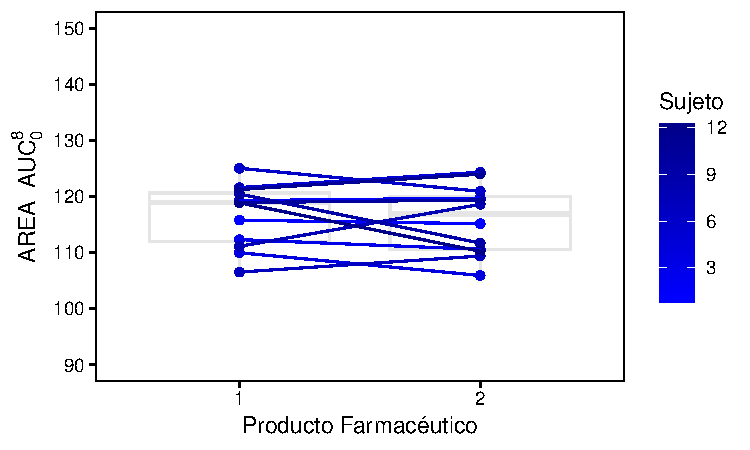
\includegraphics{parcial_1_files/figure-latex/unnamed-chunk-32-1} 

}

\caption{Comparación AUC total}\label{fig:unnamed-chunk-32}
\end{figure}

\begin{figure}[H]

{\centering 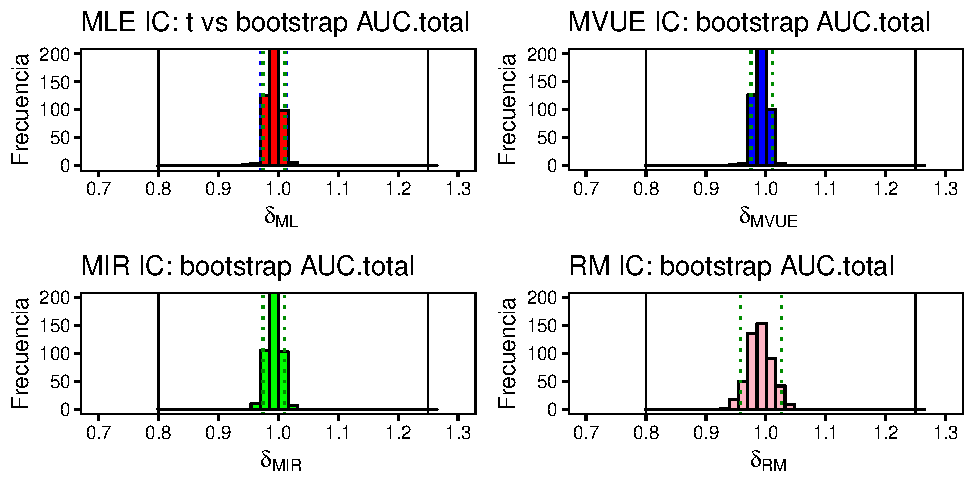
\includegraphics{parcial_1_files/figure-latex/unnamed-chunk-33-1} 

}

\caption{Estimación Diferencias AUC total}\label{fig:unnamed-chunk-33}
\end{figure}

\begin{figure}[H]

{\centering 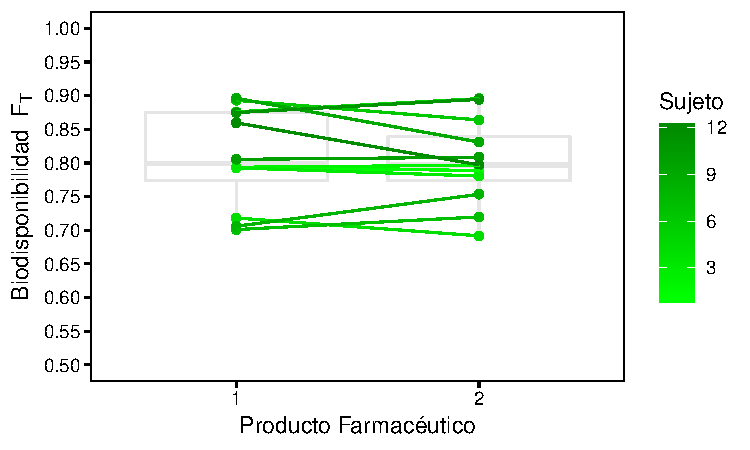
\includegraphics{parcial_1_files/figure-latex/unnamed-chunk-34-1} 

}

\caption{Comparación Biodisponibilidad (F)}\label{fig:unnamed-chunk-34}
\end{figure}

\begin{figure}[H]

{\centering 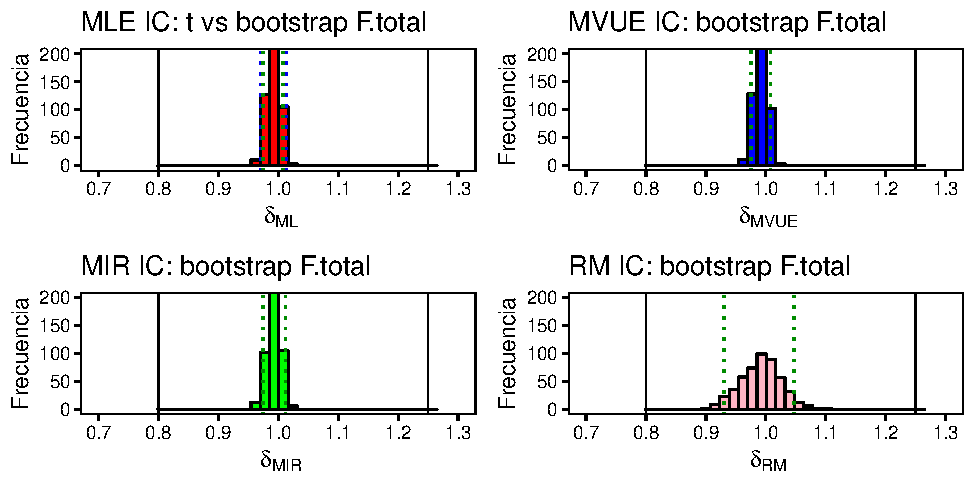
\includegraphics{parcial_1_files/figure-latex/unnamed-chunk-35-1} 

}

\caption{Estimación Diferencias F}\label{fig:unnamed-chunk-35}
\end{figure}

\begin{figure}[H]

{\centering 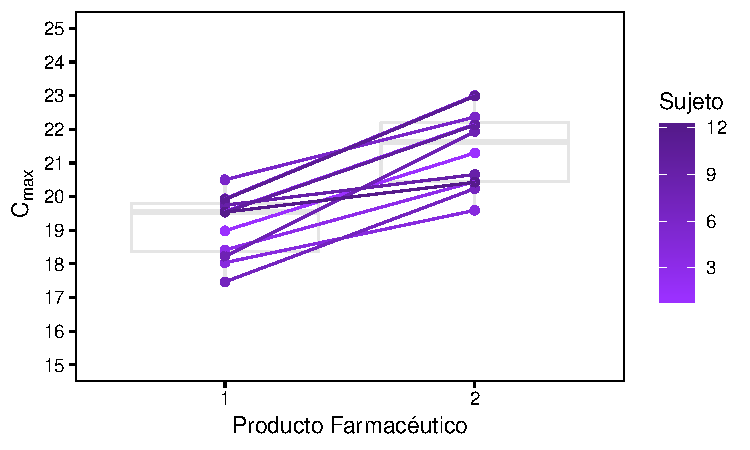
\includegraphics{parcial_1_files/figure-latex/unnamed-chunk-36-1} 

}

\caption{Comparación Cmax}\label{fig:unnamed-chunk-36}
\end{figure}

\begin{figure}[H]

{\centering 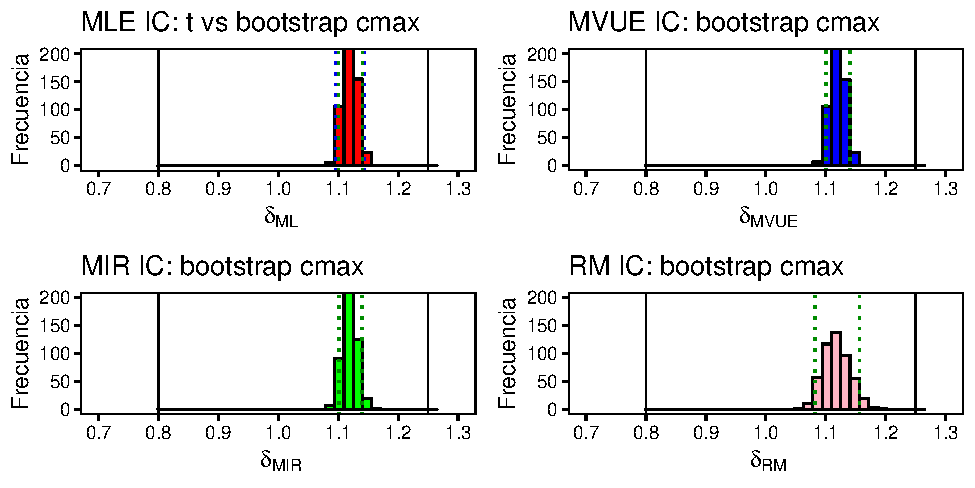
\includegraphics{parcial_1_files/figure-latex/unnamed-chunk-37-1} 

}

\caption{Estimación Diferencias C.max}\label{fig:unnamed-chunk-37}
\end{figure}

\begin{figure}[H]

{\centering 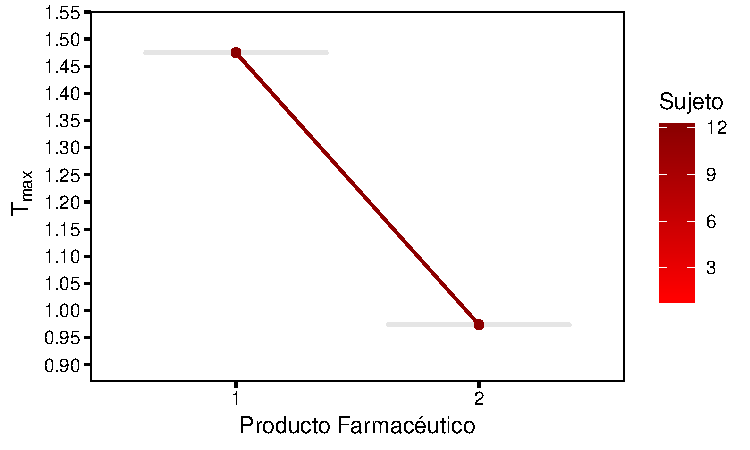
\includegraphics{parcial_1_files/figure-latex/unnamed-chunk-38-1} 

}

\caption{Comparación Tmax}\label{fig:unnamed-chunk-38}
\end{figure}

\subsection{5.6. Resultados en Pruebas no
Parámetricas}\label{resultados-en-pruebas-no-parametricas}

En la figura 15, se puede observar que hay diferencias en el parámetro
\(T_{max}\), se realiza un test de rango con signos de Wilcoxon pareado
(\(\alpha = 0.10\)) para conocer si existe diferencia en este parámetro
de acuerdo al tipo de formulación. Este parámetro tiene naturaleza
discreta y es muy dependiente del diseño del muestreo, por tal no suele
tener distribución normal ni siquiera tras transformación, y su
comparación se debe hacer de forma no paramétrica
(\protect\hyperlink{ref-Rani2004}{5}).

Se encuentra en principio que el valor para el parámetro en el producto
competidor es menor, frente a la referencia. El test de Wilcoxon muestra
un valor de estadístico V = 78, mientras el valor tabulado para ese
nivel de significancia es 61, el valor p en este caso es 4.88E-04. Por
lo cual, se rechaza la hipótesis nula de que la diferencia es igual a
cero en este parámetro. Se tiene que la diferencia es significativa para
un \(\alpha/2 = 0.05\).

No se pueden conocer los valores de todos los efectos tal como en el
tratamiento de ANOVA para medidas repetidas, ya que su equivalente es el
test de Friedmann sólo permite analizar un factor a la vez. Por lo cual,
se sabe que existe la diferencia pero no se conoce si es mayor a los
umbrales exigidos por agencias regulatorias.

\begin{figure}[H]

{\centering 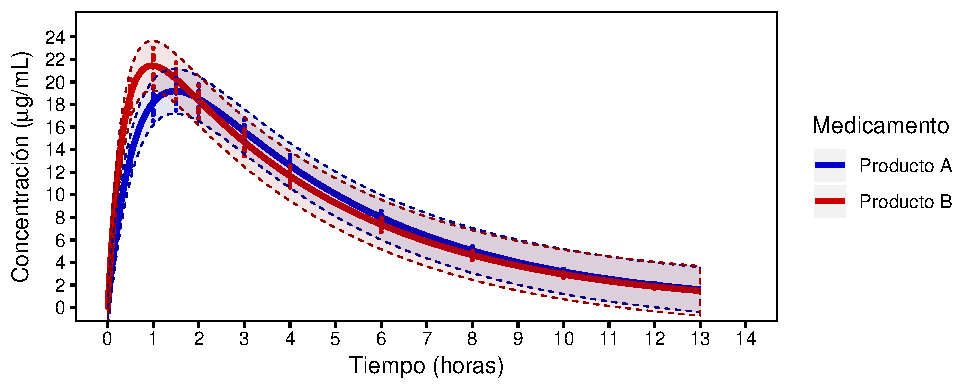
\includegraphics{parcial_1_files/figure-latex/unnamed-chunk-39-1} 

}

\caption{Perfil Promedio de Productos con IC}\label{fig:unnamed-chunk-39}
\end{figure}

\section{6. Conclusión}\label{conclusion}

Se ha determinado que existen diferencias significativas en el caso
\(C_{max}\) pero estas no sobrepasan el límite de aseguramiento impuesto
por la regla 80/125. En los parámetros de área bajo la curva total
(\(\textrm{AUC}\mid_{0}^{\infty}\)) y biodisponibilidad absoluta (\(F\))
no se determinaron diferencias significativas debidas a la formulación.

Pueden haber problemas por el efecto en la variación en seguridad y
eficacia, y esto depende del fármaco exclusivamente. Se debería evaluar
cual es el efecto de un aumento en la \(C_{max}\) sobre todo en la
seguridad del medicamento. Pese a que esta formulación se puede utilizar
de manera intercambiable con el producto de referencia, y se tiene que
existe \emph{``prescribability''} puesto que el clínico tiene la
libertad de elegir cualquiera de los dos productos en pacientes nuevos
ya que se espera el mismo efecto (\protect\hyperlink{ref-Chow2009}{2}).

Sin embargo, no se puede asegurar la \emph{``switchability''} que es la
capacidad de cambiar el producto una vez prescrito de manera libre, es
decir, en pacientes antiguos a los cuales se ha llevado el fármaco a
niveles seguros a través de titulación de la dosis. En este caso,
debería realizarse un estudio de \texttt{bioequivalencia\ individual}
para demostrarlo. De manera similar, la intercambiabilidad entre
diferentes genéricos, ya que se tiene equivalencia con el innovador pero
no con otros productos competidores en cuyo caso podrían pasarse los
límites impuestos por la regla 80/125.

En conclusión, se puede declarar \texttt{bioequivalencia\ promedio} dado
que los parámetros \(C_{max}\) y \(\textrm{AUC}\mid_{0}^{\infty}\) son
equivalentes entre producto de referencia y competidor.

\section*{7. Bibliografía}\label{bibliografia}
\addcontentsline{toc}{section}{7. Bibliografía}

\hypertarget{refs}{}
\hypertarget{ref-Olsson2005}{}
1. Olsson U. Confidence intervals for the mean of a log-normal
distribution. J Stat Educ. 2005;13(1).

\hypertarget{ref-Chow2009}{}
2. Chow S-C, Liu J-P. Design and Analysis of Bioavailability and
Bioequivalence Studies. 3rd ed. New York: Taylor \& Francis Group, LLC;
2009.

\hypertarget{ref-WorldHealthOrganization2006}{}
3. World Health Organization. Annex 7. Multisource (generic)
pharmaceutical products: guidelines on registration requirements to
establish interchangeability. 2006. pp. 131--84.

\hypertarget{ref-MinisteriodeSaludyProteccionSocial2016}{}
4. Ministerio de Salud y Protección Social. Anexo Técnico 1. Guía de
Biodisponibilidad (BD) y Bioequivalencia (BE) de Productos
Farmacéuticos: Por la cual se establece la guía de Biodisponibilidad
(BD) y Bioequivalencia (BE) y se dictan otras disposiciones. 2016. pp.
1--47.

\hypertarget{ref-Rani2004}{}
5. Rani S, Pargal a. Bioequivalence: An overview of statistical
concepts. Indian J Pharmacol. 2004;36(4):209--16.


\end{document}
